\documentclass{anvil-paper}
\usepackage{array}
\usepackage{float}
\newcommand{\Nm}{\mathrm{N\,m}}
\newcommand{\dd}{\,\mathrm{d}}
\title{Adjoint gradients reach validated torque-ripple targets\\
2.5 to 4 times sooner than finite differences\\in a nonlinear motor model}
\author{Robb Walters}
\date{October 2026}
\hypersetup{pdftitle={Adjoint gradients reach validated torque-ripple targets 2.5 to 4 times sooner than finite differences in a nonlinear motor model},pdfauthor={Robb Walters},pdfsubject={Matched optimization, torque-ripple reproduction and discrete design-gradient verification}}

\begin{document}
\maketitle
\begin{abstract}
A differentiable field model pays off in design only if its gradients
shorten the path to a design that survives independent validation. We
reconstruct a published nonlinear permanent-magnet motor in our GEODE
finite-element implementation, verify its discrete design gradients, and
compare optimizers in a preregistered, budget-matched study judged by a
common order-93 validation model. SLSQP driven by adjoint gradients reached
torque-ripple targets sooner than COBYQA at the same training resolution in
all 45 paired comparisons where both succeeded, by geometric means of
2.45--3.25 in an eight-parameter space and 3.14--7.79 in an 18-parameter
space. Because that contrast also changes the optimizer, we added a
post-hoc ablation after these outcomes were known, under a protocol frozen
before its runs: the same safeguarded SLSQP with forward-difference
gradients. With the optimizer held fixed, adjoint gradients reached the
primary target 2.47 times sooner in the eight-parameter space and 4.11
times sooner in the 18-parameter space (geometric means over five starts,
ranges 2.45--2.52 and 3.84--4.33), and both variants reached every primary
target from every start. The ratio grows with the number of parameters, as
the cost of a finite-difference gradient does, although the two spaces also
differ in mesh-motion map. Compared approximately across the two sessions,
gradient access accounts for roughly 80\% and 70\% of the logarithm of the
SLSQP-versus-COBYQA ratios, and the optimizer for the rest. Validating each
new incumbent took 53\% of all charged time in the main study and dilutes
every ratio. A coarser training mesh made runs only 1.3--2.2 times faster
and, with SLSQP, missed targets from one start in each design space. Every
selected target crossing met its target on a finer mesh, which changed the
main study's objectives by $-4.0\%$ to $+1.1\%$. Validation uses a higher
interface order than training because the ripple objective depends on it:
at the finest mesh, truncating harmonic coupling at the reference's order
45 lowers loaded torque standard deviation by 7--9\% and raises cogging
standard deviation by 59\% relative to conforming coupling.
\end{abstract}

\section{Introduction}
Whether to pay for derivatives is a practical design decision. An adjoint
gives the sensitivities of a few outputs to many design parameters at the
cost of one linear solve per output and operating state, without a field
solve per parameter \citep{scotzniovsky2025}, so a gradient-based step is
cheap once the derivatives exist. That does not settle whether following those
gradients reaches a good design sooner than a derivative-free search, or
whether the design survives a better model. The adjoint differentiates the
chosen discrete model and excitation policy; it does not establish that the
objective is resolved. In aerodynamic shape optimization an adjoint
gradient-based method has needed far fewer function evaluations than a
genetic algorithm \citep{zingg2008comparative}, so the direction of an
advantage is expected. Its size for a nonlinear motor, measured on a
validated target with failures retained, is the question here.

We answer it with a preregistered, budget-matched comparison of five
methods in two nested design spaces of a published nonlinear
permanent-magnet motor \citep{wiesheu2024spline} (Section~\ref{sec:optimization}).
Every candidate is judged by one validation model with a finer mesh and a
higher interface order than any training model, and cost is whole-run wall
time with nothing subtracted. Wherever both reach a target from the same
start, SLSQP with adjoint gradients gets there sooner than COBYQA trained on
the same mesh, by geometric means of 2.45--3.25 in the eight-parameter
space and 3.14--7.79 in the 18-parameter space. Validation charges make
these ratios conservative, but they also account for most of SLSQP's lead
over the coarse derivative-free competitor in the eight-parameter space. A
coarser training mesh speeds runs by only 1.3--2.2 times and costs
reliability, and the selected designs pass refinement checks.

That contrast changes the search strategy together with gradient access, so
by itself it does not show that the adjoint is what pays off. A post-hoc
ablation, added after the main outcomes were known and run under a
protocol frozen before its runs, holds SLSQP fixed and replaces the adjoint
by forward differences (Section~\ref{sec:exp2-fd}). The adjoint then
reaches the primary target 2.47 times sooner with eight parameters and
4.11 times sooner with 18. Gradient access is therefore the larger part of
the SLSQP-versus-COBYQA advantage, and the optimizer contributes the rest.

Two sets of checks make the comparison interpretable. First, the training
objective depends on the rotor--stator interface model
(Section~\ref{sec:forward}). Reconstructing the initial motor of
\citet{wiesheu2024spline}, we find that truncating the interface at order 45
lowers loaded torque standard deviation by 7--9\% and raises cogging
standard deviation by 59\% on the finest mesh, relative to conforming
coupling, while the loaded mean torque of either model agrees with the
saved reference within 0.16\%. This is why validation uses a higher order
than training. Second, the design gradients pass finite-difference and
Taylor checks at scalar design points and in both optimization spaces
(Sections~\ref{sec:optimization} and \ref{sec:gradients}), yet verified
ripple sensitivities differ between interface/estimator models, and holding
winding-group-1 density rather than current fixed reverses three
mean-torque sensitivities. The numerical methods are established; the
contribution is the measured time-to-target evidence for adjoint gradients,
separated from the choice of optimizer, against finite-difference,
derivative-free and coarse-model alternatives, with the checks that show
what the gradients represent.

\section{Related work}
\citet{wiesheu2024spline} combine spline-based rotor and stator shape
optimization with engineering parameters for a nonlinear permanent-magnet
synchronous motor. Their public implementation and saved outputs provide
the reproduction target here. Their related study combines parameter and
shape optimization with isogeometric analysis and compares against each alone
\citep{wiesheu2025combined}. We inherit the initial geometry, material
table and excitation conventions; we replace the field discretization and compare two
rotor--stator couplings. The resulting comparison is between numerical
models, rather than a comparison with a measured physical motor.

\citet{gangl2015shape} derive shape sensitivities of a rotor iron design
under nonlinear magnetostatics, using a shape-Lagrangian formulation, to
smooth the rotation pattern of an electric motor.
\citet{scotzniovsky2025} combine free-form deformation, differentiable
mesh warping and electromagnetic analysis with adjoint-based derivatives.
\citet{merkel2021shape} use isogeometric shape derivatives and harmonic
rotor--stator coupling to reduce electromotive-force harmonic distortion,
and validate initial and optimized designs with a separate field solver.
Here we examine torque standard deviation in a nonlinear reconstruction,
test which interface model and excitation policy its gradients represent,
and measure what following them costs.

\citet{degersem2004harmonic} formulate harmonic weighting functions at
the sliding interface of a finite-element machine model.
\citet{bontinck2018isogeometric} use separate isogeometric subdomains and
harmonic interface constraints; their exact circular geometry avoids
polygonal air-gap error, and they analyze stability as the multiplier space
grows relative to the field space. \citet{egger2022torque} derive torque from the
energy of a harmonic mortar formulation and examine its numerical
accuracy for ripple evaluation. Their linear-material cogging experiment
varies the maximum transmitted order from 39 to 129 and compares against
a refined order-200 reference. Thus torque sensitivity to interface order
is already established; our study quantifies its effect on loaded nonlinear
ripple, a saved optimized design, and design sensitivities. We compare
coupling torque with the gap-averaged stress expression of
\citet{arkkio1987}. The sensitivity of cogging-torque prediction to
finite-element discretization and evaluation method was examined by
\citet{howe1992cogging}; \citet{arkkio2012proper} study mesh selection for
torque computation.

\citet{duan2013review} review surrogate, direct and stochastic
search for machine design and compare response-surface and
differential-evolution methods on a five-variable permanent-magnet motor
benchmark, so neither arm uses gradients; \citet{bramerdorfer2018modern} survey optimization scenarios and
techniques for electrical machines. \citet{ion2018robust} compare
deterministic gradient-based optimization with stochastic search for
electric devices, including a permanent-magnet motor, using geometry
parametrizations that avoid remeshing. \citet{zingg2008comparative} found
that a genetic algorithm needed 5 to 200 times as many function
evaluations as an adjoint gradient-based method in aerodynamic shape
optimization, depending on the problem, the number of design variables and
the degree of convergence. Section~\ref{sec:optimization} adds a matched
measurement of this kind for a nonlinear motor, with a coarse
finite-element competitor, a common validation target and wall time as the
cost. Its time-to-target measure follows the performance profiles of
\citet{dolan2002benchmarking} and the data profiles that
\citet{more2009benchmarking} developed for derivative-free solvers, here
with a fixed wall-time budget and censored targets.

\citet{kemmetmueller2015} use nonlinear magnetic equivalent circuits for
torque control, including saturation and nonsinusoidal behavior. Their
control problem differs from shape optimization, but it demonstrates why
saturation alone does not establish the need for a full-field model.
\citet{roomi2022} develop a waveform-targeting surrogate for electrical
machine design, while \citet{wen2023} adapt reduced models along a
shape-optimization trajectory in fluid examples. These approaches motivate
waveform-aware and adaptive baselines. Their published performance is not
transferred to the motor studied here.

\section{Motor model}\label{sec:model}
\subsection{Geometry and operating states}
The full machine has six poles and 36 stator slots. We model a
$60^\circ$ sector, occupying $60^\circ\leq\theta\leq120^\circ$ at zero
rotation, with antiperiodic conditions on the radial boundaries. The rotor
inner and outer radii are 16 and 44\,mm; the stator inner and outer radii
are 45 and 67.5\,mm. Axial length is $L=0.1$\,m. The 1\,mm air gap is
split at the coupling radius $r_c=44.5$\,mm. Figure~\ref{fig:geometry}
shows the material-tagged reconstruction.

\begin{figure}[htbp]
\centering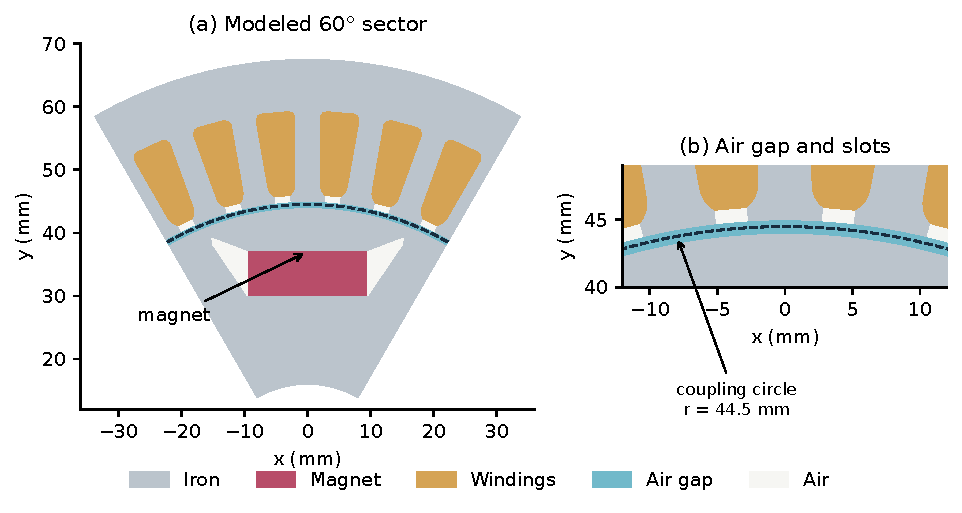
\includegraphics[width=\linewidth]{figures/geometry.pdf}
\caption{Initial-design geometry rendered directly from the committed
coarsest mesh. The dashed line is the rotor--stator coupling circle. The
right panel enlarges the gap and slot openings. Material boundaries are
shown without the element edges; the geometry is not an optimized result.}
\label{fig:geometry}
\end{figure}

The reconstruction uses the initial NURBS exports in the public snapshot.
Their control points are stored with weights already multiplied in, and
patch orientation must be accounted for when integrating areas. Two thin
rotor patches described as air slits in source comments receive iron under
the reference's material assignment; we follow that assignment. The
mesh generator, built on Gmsh 4.15.2 \citep{geuzaine2009gmsh}, preserves the winding groups
separately, since their two characteristic areas are approximately 36.29
and 31.22\,mm$^2$.

At mechanical angle $\beta$, phase currents are
\begin{equation}
 I_q(\beta)=a I_*\sin(\phi_0+3\beta+\delta_q),\qquad
 (\delta_U,\delta_V,\delta_W)=(0,-2\pi/3,2\pi/3),
 \label{eq:current}
\end{equation}
where $a\in\{0,0.5,1\}$, $I_*=9.677657374$\,A, and the electrical phase
offset $\phi_0=0$ for the initial design. Angles in
Eq.~\eqref{eq:current} are in radians. Each winding group carries current
density $J_g=12s_g I_q/|\Omega_g|$, with its own area and prescribed sign
$s_g\in\{-1,1\}$. Using a common area would change the current density
between groups by about 16\%. We compare 20 distinct mechanical angles,
$0^\circ,1^\circ,\ldots,19^\circ$, excluding the duplicated endpoint in
the source CSV. The reference's optimization grid contains the ten even
angles; both grids are retained in the artifacts.

\subsection{Field model and rotor--stator coupling}
We solve two-dimensional nonlinear magnetostatics for the vector potential
$A_z$ with continuous piecewise-linear triangles and a tabulated M27 iron
law, using Newton's method with the consistent material tangent. The rotor
and stator meet at the coupling circle in one of two ways: a conforming
interface identifies matching trace nodes after rotation, while the
harmonic model, following the reference, imposes trace continuity only for
the orders $n=3,9,\ldots,N_h$ through Lagrange multipliers, with
$N_h=45$ unless stated otherwise. Torque is evaluated either by the
gap-averaged Arkkio expression \citep{arkkio1987} or, for the harmonic
model, by the coupling torque from the constrained energy derivative
\citep{egger2022torque}. Forward comparisons use Arkkio for both couplings
to isolate the interface change; the derivative study pairs harmonic
coupling with coupling torque and conforming coupling with Arkkio; the
optimization study trains on order-45 coupling torque and validates on
order 93. Retaining every order below the trace Nyquist limit reproduces
the conforming Arkkio torques within $4.1\times10^{-9}$\,N\,m on L0 and
$1.3\times10^{-9}$\,N\,m on L1, without fitting any parameter to the saved
torque. Appendix~\ref{sec:fieldmodel} gives the weak form, tangent, iron
law, coupling constraints and torque expressions.

\subsection{Meshes and statistics}
The study uses four meshes, L0--L3, with 3,153, 9,937, 36,083 and
139,268 nodes. The $60^\circ$ coupling arc has $120\cdot2^\ell$ segments at level
$\ell$, so integer-degree rotation is represented at every level.
A solution at one angle initializes the next angle at the same current.
We report the mean and population standard deviation,
\begin{equation}
 \bar T=\frac1N\sum_{k=1}^N T_k,\qquad
 \sigma_T=\left[\frac1N\sum_{k=1}^N(T_k-\bar T)^2\right]^{1/2},
 \quad N=20.
\end{equation}
The standard deviation is the ripple metric. At zero current it measures
cogging, the torque variation caused by the permanent magnets and slots
without applied phase current. The squared-ripple objective is
$F=\sum_{a\in\{0,0.5,1\}}\sigma_T(a)^2$, in $\mathrm{N^2\,m^2}$, on the
20-angle grid. Appendix~\ref{sec:fieldmodel} lists the implementation checks.

\section{Matched optimization study}\label{sec:optimization}
This section tests whether adjoint-driven optimization shortens the time
needed to reach a common validated ripple target. The protocol and all of
its amendments were fixed in the
\href{https://github.com/rjwalters/geode-fem/issues/1185}{preregistration}
before any main-run outcome was observed. One later deviation, in how the
final refinement was run, was adopted after the main runs had finished and
is described with the refinement in Section~\ref{sec:exp2-refinement}; it
changes no selection rule, check or target. The finite-difference ablation
of Section~\ref{sec:exp2-fd} was added after the main outcomes were known
and is not part of the preregistered study.

\subsection{Protocol}
\paragraph{Methods.}
Five methods form an optimizer-by-resolution comparison plus one
surrogate (Table~\ref{tab:methods}). A and E are SLSQP
\citep{kraft1988} using the field adjoints of Section~\ref{sec:gradients},
safeguarded so that a refused request restores the last admissible point
and restarts the solver; B and D are COBYQA \citep{ragonneau2022} with $2n+1$ interpolation points
and unit-box trust radii $0.1$ to $10^{-6}$, where $n$ is the number of free
parameters. Both run through SciPy 1.18.1 \citep{virtanen2020scipy}. C is
an empirical trust-region method on four cubic radial-basis interpolants
of the L1 training outputs (the three per-current standard deviations and
the full-current mean), refitted after every evaluation from an $n+1$-point
initial design; Appendix~\ref{sec:settings} gives its radii, acceptance
and update rules and the other settings. A/B and E/D vary the optimizer at fixed training resolution,
and A/E and B/D vary resolution at fixed optimizer. The optimizer contrast
includes differences in search strategy, so it does not isolate gradient
access as the only causal difference. Training uses order-45 coupling torque
on 20 angles at current fractions $0$, $\tfrac12$ and $1$ of the fixed peak
current $9.6777\,\mathrm{A}$. L0 and L1 differ only in spatial resolution,
and neither is fitted or corrected against validation. Time to a fixed
target, with unattained targets kept as censored, follows the data- and performance-profile
practice for benchmarking optimization solvers \citep{more2009benchmarking,dolan2002benchmarking}.
The preregistration also named a fixed group-1 current-density rule as a
labelled control. It was not run in this study, which uses the fixed
physical current throughout; Section~\ref{sec:gradients} reports that
rule's effect on sensitivities.

\begin{table}[H]\centering\small
\caption{Methods. D and E solve the coarse nonlinear field equations; they
are neither fitted magnetic circuits nor reduced-basis models.}
\label{tab:methods}
\begin{tabular}{lll}\toprule
Method & Optimizer or search model & Training mesh\\\midrule
A & Safeguarded SLSQP, field adjoints & L1\\
B & COBYQA, forward evaluations & L1\\
C & Empirical cubic-RBF trust region & L1\\
D & COBYQA, forward evaluations & L0\\
E & Safeguarded SLSQP, field adjoints & L0\\\bottomrule
\end{tabular}
\end{table}

\paragraph{Design spaces and constraints.}
Space A has eight free geometric lengths: MAG, MH, MW, SW1--SW4 and Sr1
(Appendix~\ref{sec:parameters}), that is, the rotor iron depth, magnet
height and width, four stator tooth and slot dimensions, and the slot-bottom
fillet radius. Space B adds ten grouped offsets acting on 55 surface control
points. Stack length, radial scale, stator outer diameter and operating
angle are fixed, so the saved Opt120 design lies outside both spaces. The
two spaces also use different discrete mesh-motion maps, so their contrast
does not isolate the ten added offsets.
Each training model $r\in\{\mathrm{L0},\mathrm{L1}\}$ minimizes
$F_r=\sum_c\sigma_{r,c}^2$ over the three training currents, subject to
$\mu_{r,1}\geq1.0025\,\mu_{r,1}(\theta_0)$ for its own full-current mean and to
normalized construction margins $c_i-0.05\geq0$. Unbuildable or
mesh-infeasible candidates are refused: SLSQP restores toward the last
admissible point and restarts, COBYQA receives a NaN barrier, and C skips
the point. A moved mesh with an inverted triangle or a minimum angle below
$5^\circ$ is repaired by up to four charged remeshing attempts. Because
refinement cannot remove a limiting geometric corner, the $5^\circ$ policy
also acts as an implicit geometric constraint. Space B's slot-opening
channel wall is not guarded and can become very thin at extreme offsets;
that risk is handled by repair and refusal, not by a wall-thickness
constraint.

\paragraph{Training gradients.}
Section~\ref{sec:gradients} verifies a different, scalar parameter set; the
gradients that A and E use were checked separately. In both spaces, the L1
training objective $F$ and full-current mean were compared with central
differences at $\theta_0$ and at an interior point, along a fixed
box-scaled direction and for three (space A) or four (space B) components,
including the offsets CPR1 and CPS1. With Newton tolerance $10^{-12}$, the
directional relative errors at $h=10^{-4}$ are $1.5\times10^{-8}$ to
$2.8\times10^{-7}$ for $F$ and $2.4\times10^{-9}$ to $4.7\times10^{-9}$ for
the mean, and the component errors at $h=10^{-6}$ are at most
$2.8\times10^{-6}$. The directional error falls by 72 to 156 times from
$h=10^{-3}$ to $10^{-4}$, as truncation error should. The evaluator's own
gradient replies at the study's training tolerance of $10^{-8}$ agree at
the interior point within $3.1\times10^{-6}$ directionally; the largest
component error, $4.3\times10^{-5}$, belongs to the small Sr1 derivative.
At $\theta_0$, space B's offsets sit on their bounds, so the central
stencils there step outside the design box. The records are pinned with the
optimization harness (Code and data availability).

\paragraph{Common validation and credit.}
Every method is judged on the same order-93, L2, 20-angle validation model.
Its initial-design anchor is $F_0=9.6034\times10^{-3}\,\mathrm{N^2\,m^2}$ with
full-current mean $\mu_0=1.44084\,\Nm$. The targets are $T_{50}=0.5F_0$,
$T_{90}=0.1F_0$ and $T_{99}=0.01F_0$. A validated design attains a target
only if
\begin{equation}
 F_{\mathrm{val}}+\delta F\leq T,\qquad
 \delta F=\max\{0.10F_{\mathrm{val}},\,2.5\times10^{-7}\,\mathrm{N^2\,m^2}\},
\end{equation}
its validated full-current mean is at least $1.0025\,\mu_0$, its
construction margins and mesh checks pass, and its validation completes
within budget. The allowance $\delta F$ is an empirical margin, not a bound
on continuum error. Optimizer success flags confer no credit. Changed
incumbents are validated as they appear, after the initial interpolation
set for B, C and D.

\paragraph{Budget and timing.}
Cost is wall time, in units of the median cold validation forward measured
on the same host at the same concurrency. Each run receives 120 units,
with a 60-unit checkpoint that counts only validations completed by then.
The charge covers evaluator start-up, geometry checks, mesh motion and
repair, training solves, adjoints, optimizer overhead, surrogate fitting
and validation; nothing is subtracted as overhead. L0 receives no discount.

\paragraph{Starts and execution.}
Each space uses $\theta_0$ and four Latin-hypercube starts (seeds 1--4),
with the scalar coordinates matched across spaces. A start was eligible
only if it was buildable and admissible, and its moved reference mesh met
the mesh policy without repair, in both spaces at L0 and L1. The starts
therefore favor moderate deformations and are not uniform samples of the
design box. All starts were frozen before any main outcome. Every method
runs from every start twice, giving 100 runs. Within a start, repeat 1
rotates the method order and repeat 2 reverses it.

The session ran on one AWS c7a.4xlarge host (x86-64; NumPy 2.5.4 and
SciPy 1.18.1 with OpenBLAS) with 15 concurrent single-threaded processes.
Before calibration, the host recomputed the initial-design validation
waveforms in both spaces. $F_0$ agreed with the canonical anchor to
$2.4\times10^{-13}$ relative, within the preregistered $10^{-9}$ tolerance,
and the two spaces agreed bit for bit. The calibrated unit was
$70.94\,\mathrm{s}$, the median of 45 concurrent cold validations. All 100
runs completed in one session with no recovery, deferral or contamination:
the one-minute load average peaked at 21.1, below the contamination
threshold of $1.5N=22.5$. The in-run cost totals 109~CPU-hours. Of the
100 runs, 38 stopped on reaching $T_{99}$, 46 on optimizer convergence and
13 at the budget. The other three are SLSQP runs (A) in space A whose
solver stopped without converging: both repeats from LHS~2, after about 43
units, and repeat~1 from LHS~3, after 119 units.

\subsection{Results}
\paragraph{Repeats.}
The two repeats of each run follow the same optimization path. In all 50
pairs, the sequences of validated objectives agree exactly up to the
shorter run's length, and they differ in length only when the budget or a
solver stop cuts one repeat earlier. The repeats therefore measure timing
noise, not independent outcomes, and the comparison is a paired case study
over five starts. Over the 111 target crossings attained in both repeats,
the time differs by a median of 2.1\% and at most 12.4\% relative to
repeat~1. Repeat-1 times are reported below.

\paragraph{Attained quality.}
Figure~\ref{fig:exp2-quality} shows the best credited value of
$(F+\delta F)/F_0$ for every start, method and space (repeat~1).
In space A, no run goes below $F/F_0=0.043$ and none reaches $T_{99}$.
The best designs of A, B, D and E all reach $0.043F_0$, and C's reaches
$0.049F_0$; in Fig.~\ref{fig:exp2-quality}, which includes the allowance,
the A, B, D and E level appears near $0.048$ (C's near $0.054$). All five lie within 0.17\% above the
full-current mean floor, so the mean constraint is active there: the level
shared by A, B, D and E is the constrained optimum they found in the
eight-parameter space,
not a property of any one method. In space A the start mattered more than
the method. From LHS~4, A and B stop near $0.09F_0$, D reaches $0.044F_0$,
and C and E never produce a credited validation, in either repeat. In
space B, each method's best design reaches $0.004$--$0.009F_0$, and every
method except C reaches $T_{99}$ from at least four of five starts.

\begin{figure}[t]\centering
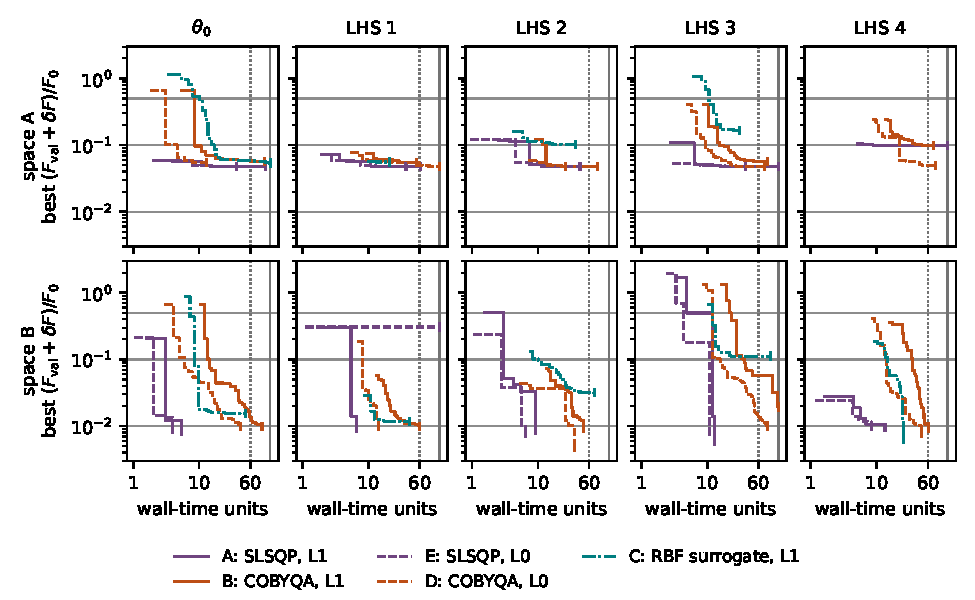
\includegraphics[width=\linewidth]{figures/exp2-quality.pdf}
\caption{Best credited $(F_{\mathrm{val}}+\delta F)/F_0$ versus charged wall
time, repeat~1, at common L2/order-93/20-angle validation. Grey lines mark
$T_{50}$, $T_{90}$ and $T_{99}$; the dotted and solid vertical lines mark
the 60-unit checkpoint and the 120-unit budget. The time axis is
logarithmic. Each curve ends at the run's actual stop (tick). A missing curve
means the run had no credited validation.}
\label{fig:exp2-quality}
\end{figure}

\paragraph{Time to target.}
Figure~\ref{fig:exp2-time} gives the charged time to each target, per
start, and Table~\ref{tab:exp2-time} in Appendix~\ref{sec:exp2-times} lists
the values. In repeat~1, only three crossings occur
after the 60-unit checkpoint, all at $T_{99}$ in space B: two by B and one
by D.

Table~\ref{tab:exp2-ratios} (Appendix~\ref{sec:exp2-times}) gives paired time ratios. A ratio is formed
only when both methods attain the target from that start; no finite ratio
is derived from a censored cell. Wherever both reach a target from the
same start, gradient-based SLSQP gets there sooner than COBYQA at the same
training resolution. At L1 (B/A), the geometric-mean ratio is 3.10--3.25 in
space A and 5.06--7.79 in space B. At L0 (D/E), it is 2.45--2.75 and
3.14--7.20.
All 45 finite optimizer-contrast pairs (by space, target and start) favor
SLSQP, with ratios from 1.46 to 21.5. The coarse mesh shortens the time by
a smaller factor: the geometric-mean E/A ratio is 0.62--0.79 and D/B is
0.45--0.56. As charged, A is faster than D, the inexpensive derivative-free
physical competitor, by a geometric mean of 1.68--1.83 in space A and
2.25--4.32 in space B. This contrast changes both factors; one of its 25
pairs is a near tie (0.99, space-A LHS~2 at $T_{90}$: D is 0.75\% faster,
within the timing noise between repeats), and in space A most of the
contrast comes from validation charges (next paragraph). We conjecture that part of the larger
space-B ratios comes from COBYQA's initial interpolation set, which costs
$2n+1=37$ training evaluations before its first model step there, against
17 in space A.

\paragraph{Validation charges.}
Validating every new incumbent makes validation the largest single
charge (Table~\ref{tab:exp2-validation}). One validation costs a median of
0.87 units over the 3,350 completed validations (range 0.55--1.10), and
validation takes 53\% of all charged time, 2--90\% per run. SLSQP crosses
a target after few validations, but most of its time to a target is
validation; COBYQA at L1 (B) needs more validations, which are a smaller
part of its time. Excluding the validation charges up to each crossing, the
same-resolution geometric means rise to 5.41--5.66 (B/A) and 5.55--5.56
(D/E) in space A, and to 8.84--13.58 and 7.92--15.27 in space B, so the
ratios as charged are conservative for the optimizer contrast. The coarse
mesh cuts the remaining time more, by geometric means of 0.19--0.27 (E/A)
and 0.20--0.23 (D/B), but it does not make validation cheaper, which is why
its overall saving is only 1.3--2.2 times. The space-A contrast between A
and D does not survive this decomposition: excluding validation, its
geometric mean is 1.15--1.16, and two of its ten space-A pairs favor D
(0.97 and 0.54). In space A, A's lead over D therefore reflects mainly how
many validated incumbents each method needs before crossing under the
validate-every-incumbent rule (medians of two and six). In space B the
non-validation D/A mean remains 1.92--3.19.

\begin{table}[tbp]\centering\small
\caption{Validation charges, repeat~1. ``To crossing'' counts the
validations up to and including the first attaining one, and ``share''
gives the fraction of the time to that target charged to validation, as
medians (ranges) over the method's attained targets and starts. ``Run''
gives the range over starts of the fraction of the whole run's charged time
spent in validation.}
\label{tab:exp2-validation}\begin{tabular}{lllllll}\toprule
 & \multicolumn{3}{c}{Space A} & \multicolumn{3}{c}{Space B}\\\cmidrule(lr){2-4}\cmidrule(lr){5-7}
Method & To crossing & Share & Run & To crossing & Share & Run\\\midrule
A & 2 (2--7) & 0.65 (0.65--0.71) & 0.45--0.71 & 3 (1--10) & 0.61 (0.58--0.68) & 0.65--0.68\\
B & 5 (2--25) & 0.46 (0.22--0.53) & 0.24--0.34 & 8 (2--36) & 0.34 (0.15--0.45) & 0.35--0.49\\
C & 6.5 (2--10) & 0.53 (0.42--0.64) & 0.02--0.63 & 4 (2--17) & 0.40 (0.25--0.56) & 0.50--0.61\\
D & 6 (2--20) & 0.81 (0.60--0.84) & 0.41--0.64 & 9 (2--70) & 0.71 (0.46--0.77) & 0.73--0.77\\
E & 2 (1--5) & 0.90 (0.87--0.92) & 0.82--0.90 & 3 (1--11) & 0.88 (0.83--0.90) & 0.87--0.90\\
\bottomrule\end{tabular}

\end{table}

The speed of E has a reliability cost. E never produces a credited
validation from space-A LHS~4. From space-B LHS~1 it reaches $T_{50}$ but
then stalls at $0.28F_0$, missing $T_{90}$ and $T_{99}$. In four
start--target cells, D reaches a target that E misses. A, by contrast,
reaches every target that any method reaches, from every start. C attains
$T_{99}$ only once in space B and reaches $T_{90}$ from two of five
space-A starts.

\begin{figure}[t]\centering
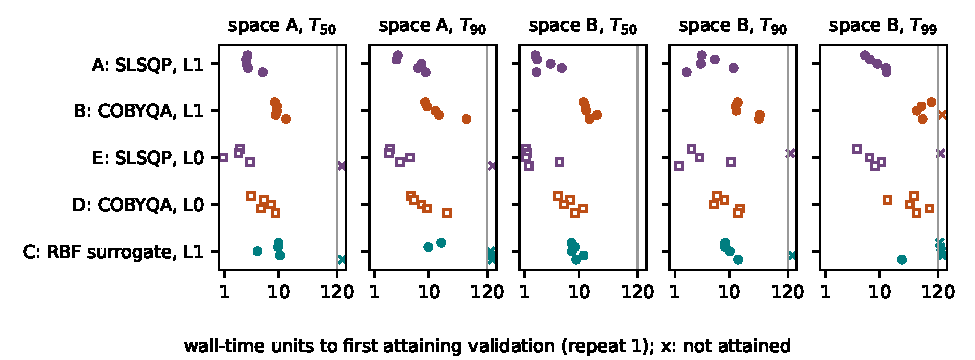
\includegraphics[width=\linewidth]{figures/exp2-time-to-target.pdf}
\caption{Charged wall time to the first attaining validation, repeat~1, one
marker per start, for every target attained by some run. Filled markers:
L1 training; open markers: L0 training; crosses: not attained within 120
units.}
\label{fig:exp2-time}
\end{figure}

\paragraph{Final refinement.}\label{sec:exp2-refinement}
The preregistered selection takes, for each method and space, the
lowest-$F_{\mathrm{val}}$ feasible design over both repeats, and the
earliest repeat-1 crossing of each attained target. With $\theta_0$ in
each space and identical designs merged, this gives 33 designs. Each
received the six registered checks: the primary L2 validation, L3, a
40-angle grid, Newton tolerance $10^{-12}$, an independently solved grid
shifted by $0.5^\circ$, and held-out currents $0.25$ and $0.75$. The 15
designs with zero stator offsets also received the conforming outer-band
Arkkio check on fresh meshes. All 213 checks completed
(Table~\ref{tab:exp2-refinement} in Appendix~\ref{sec:exp2-times}). These checks qualify the selected
designs only; they do not check each of the study's 111 repeat-1
target crossings.

The registered pipeline begins by capturing the closed study on its
original host, a step that could not be completed after that host had been
restarted. The refinement instead used a copy of the study outputs whose
integrity is established by a SHA-256 inventory of every output file, taken
when the session finished, and independently timestamped; the timestamps
establish that the inventory existed by 2026-10-20 03:50~UTC. It ran on a different host (Apple M3 Ultra,
macOS arm64). For the 16 selected designs validated on the moved reference
mesh, the primary check reproduces the study's $F_{\mathrm{val}}$ to below
$2.2\times10^{-12}$ relative. The other 15 candidates needed a fresh mesh,
which Gmsh triangulates differently on the two platforms; their $F$
differs by at most $1.7\times10^{-3}$ relative. The remaining two designs
are $\theta_0$ in each space, which reproduces $F_0$. The fresh-mesh
differences measure the sensitivity of $F$ to remeshing and are far below
the 10\% allowance $\delta F$.

Spatial refinement is the largest change. Over all 33 designs, L3 moves
$F$ by $-4.0\%$ to $+6.3\%$. Over the 25 target crossings alone, the range
is $-4.0\%$ to $+1.1\%$. The largest increase belongs to the overall best
design, D's in space B, whose $F$ rises from $0.0044F_0$ to $0.0047F_0$.
Angular and nonlinear effects are small: the 40-angle and shifted grids
change $F$ by at most $0.11\%$, and the tighter Newton tolerance by less
than $1.1\times10^{-5}$ relative. The conforming estimator gives $1.1\%$ to
$4.4\%$ more ripple than the order-93 coupling on the space-A designs, and
$2.0$--$2.1\%$ more at $\theta_0$. All 25 target crossings still satisfy
their target, allowance included, at L3; the smallest remaining margin is
1.2\% of the target. Every candidate also satisfies the full-current mean
floor in the primary, L3, 40-angle, tight and shifted checks, the closest
by 0.012\%. The refinement therefore confirms the selected crossings and
leaves the time-to-target comparison unchanged.

The held-out currents test the ripple reduction outside the three training
currents. We compare each design's objective at currents $0.25$ and $0.75$,
relative to $\theta_0$'s at the same currents, with its relative objective
at the training currents. Across the candidates, the held-out ratio is 0.65
to 1.73 times the training-current ratio; values above one mean a smaller
reduction at the held-out currents. For the five best space-A designs it
is 1.07--1.09. In space B, four of the five best designs keep less of
their reduction: their remaining objective fraction at the held-out currents
is 1.23--1.73 times that at the training currents, while for B's best
design it is 0.89. D's best design has $0.0044F_0$ at the training currents but
$0.0076$ of $\theta_0$'s value at the held-out currents. Part of the extra
reduction from space B's added freedom is therefore specific to the three
training currents.

The training model also reads lower than validation. At $\theta_0$, the
order-45 training objective is 0.887 (L1) and 0.894 (L0) of $F_0$. At the
31 selected designs, the ratio of training to validation objective lies
between 0.57 and 1.19 times its $\theta_0$ value. The lowest values belong
to space-B designs near $T_{99}$: E's and A's $T_{99}$ crossings (0.57 and
0.71) and D's best design (0.65); the best space-B designs of B and C are at
0.99 and 1.19. Large reductions therefore often, but not always, come with a
training objective that underestimates validation more than at $\theta_0$.
This is consistent with the cancellation conjecture of
Section~\ref{sec:opt120} but does not establish it.

\subsection{Post-hoc ablation: finite-difference SLSQP}\label{sec:exp2-fd}
The contrasts above vary the optimizer together with gradient access. This
ablation varies gradient access alone. It was added after the main
outcomes were known, so it is post hoc and not part of the preregistered
study; its protocol was frozen in a
\href{https://github.com/rjwalters/geode-fem/issues/1218}{separate public protocol}
before any of its runs.

\paragraph{Protocol.}
Method F is the safeguarded SLSQP of A with identical bounds, constraints,
restoration, validation policy, targets, mean floor and stopping rules.
Only the gradients of the objective and of the mean constraint change: they
are forward differences of training values with a step of $10^{-6}$ in each
component's unit, reusing the base value, so one gradient costs $n+1$
training forwards ($n=8$ in space A and 18 in space B). A component whose
forward step is inadmissible or would remesh uses the backward step; if
both fail, the gradient is refused as it would be for A. Every
difference solve is charged to the run. The geometry-constraint Jacobians
remain analytic, as for A. To make the comparison within one session, A is
rerun unchanged in the same session as A$'$: both methods run from the five
starts above, in both spaces, with two repeats and rotated method order,
giving 40 runs of 120 units on the L1 training model. The primary estimand
is, per start, the repeat-1 ratio F/A$'$ of time to $T_{90}$ in space A and
to $T_{99}$ in space B; a censored cell gives no finite ratio. The
representative and earliest crossings of F receive the six refinement
checks above.

\paragraph{Results.}
Per-start F/A$'$ time ratios and their geometric means: [PENDING exp2b-fd-slsqp].
Hit fractions and censoring of F and A$'$: [PENDING exp2b-fd-slsqp].
Consistency of A$'$ with the main-study A and repeat-2 reproducibility:
[PENDING exp2b-fd-slsqp].
Final refinement of F's selected designs: [PENDING exp2b-fd-slsqp].

\paragraph{Gradient credit.}
[PENDING exp2b-fd-slsqp]


\section{Interface order and the ripple objective}\label{sec:forward}
This section explains why the validation model of
Section~\ref{sec:optimization} differs from its training models. Each mesh
level contains 60 baseline solves: three current levels and 20 angles. For
a scalar statistic $q$, the estimated L3 refinement interval is
\begin{equation}
 q_3\ \pm\ e_q,\qquad
 e_q=\max\{|q_2-q_1|,|q_3-q_2|\}.
 \label{eq:band}
\end{equation}
We use the same construction pointwise for waveforms. This interval is a
refinement diagnostic, not a proven error bound or a statistical confidence
interval. It does not cover reference-model error or angular quadrature
error. The loaded means change direction between the last two increments,
so a last-increment estimate alone would be particularly weak.

\subsection{Coupling changes the ripple objective}\label{sec:coupling-results}
Table~\ref{tab:torque} compares the same geometry, material and excitation
with two interface models. The conforming L3 means are 0.15\% and 0.16\%
low at half and full current. Harmonic coupling reduces the mean deviations
to $-0.002\%$ and $+0.051\%$, with both reference means inside the estimated
refinement intervals. The loaded ripple deviations fall from $+9.9\%$
and $+11.3\%$ to $+1.7\%$ and $+1.3\%$.

\begin{table}[htbp]\centering\small
\caption{L3 population standard deviation and mean torque, in N\,m per
sector, on the 20-angle grid. The last column gives ripple deviation from the
saved reference; n/a identifies the reference itself. The reference is
subsequently refined in Section~\ref{sec:refinement}.}
\label{tab:torque}
\begin{tabular}{llrrr}\toprule
Current fraction & Model & Mean & Std & Std vs ref. (\%)\\\midrule
0 & Reference & 0.00010 & 0.01071 & n/a \\
0 & Conforming & 0.00001 & 0.00760 & $-$29.1 \\
0 & Harmonic & 0.00000 & 0.01209 & +12.9 \\
0.5 & Reference & 0.66208 & 0.03895 & n/a \\
0.5 & Conforming & 0.66106 & 0.04279 & +9.9 \\
0.5 & Harmonic & 0.66206 & 0.03961 & +1.7 \\
1 & Reference & 1.44248 & 0.07935 & n/a \\
1 & Conforming & 1.44023 & 0.08829 & +11.3 \\
1 & Harmonic & 1.44322 & 0.08036 & +1.3 \\
\bottomrule\end{tabular}

\end{table}

Figure~\ref{fig:waveforms} in Appendix~\ref{sec:controls} shows the improvement angle by angle. The largest
full-current difference falls from 0.0272 to 0.0034\,N\,m. The harmonic
full-current ripple interval contains the saved reference; the saved half-current
value lies approximately $5\times10^{-5}$\,N\,m below its interval.
Mean agreement is therefore insufficient to characterize waveform accuracy.

The saved zero-current reference exposes a separate discretization effect. Harmonic coupling changes the
cogging standard deviation from 29.1\% below to 12.9\% above the reference.
Its waveform is close to a 1.13-fold scaling of the saved waveform, but the
reference lies outside the estimated ripple interval. This motivates
refining the reference itself before interpreting the discrepancy. The harmonic cogging standard deviations are
0.0101, 0.0119, 0.0121 and 0.0121\,N\,m on L0--L3, compared with
0.0107\,N\,m in the reference. The independent reference refinement below tests this coarse-model
explanation directly.

\subsection{Spatial resolution and transmitted order}
Spatial refinement at fixed order and order refinement on a fixed mesh
answer different questions (Fig.~\ref{fig:convergence}). At L3, order 45
raises cogging standard deviation by about 59\% and lowers loaded
standard deviation by 7--9\%, relative to the conforming values. At L1 and L2,
order 189 approaches the conforming torque to within $1.1\times10^{-4}$\,N\,m.
A spatially refined order-45 solution thus remains a solution of a
truncated interface model. Matching that truncation improves reproduction
of the published calculation; it does not establish which model better
represents the physical motor.

\begin{figure}[!t]\centering
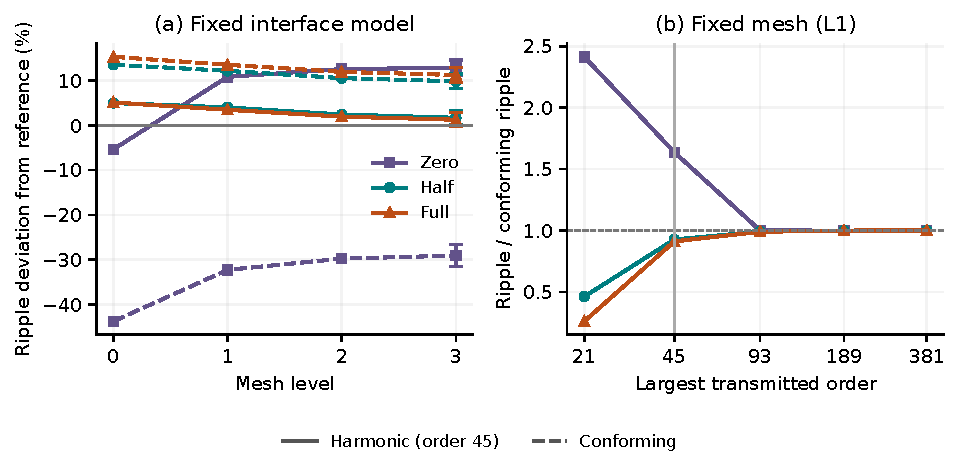
\includegraphics[width=\linewidth]{figures/coupling-convergence.pdf}
\caption{Left: ripple deviation from the reference under spatial
refinement, with solid lines for harmonic order 45 and dashed lines for
conforming coupling; L3 bars use Eq.~\eqref{eq:band}. Right: order
refinement on L1 with logarithmic order spacing, normalized by the
conforming ripple at that same level.
The saved reference uses order 45; see Section~\ref{sec:refinement} for its
refinement. Colors identify current, not coupling.}
\label{fig:convergence}\end{figure}

Two additional controls narrow the explanation. At L3, coupling torque
and the inner- and outer-half Arkkio estimates are each within
$9\times10^{-5}$\,N\,m of full-band Arkkio in the order-45 solution.
Freeing the coupling-arc ends changes torque by less than
$5.4\times10^{-5}$\,N\,m. These effects, and the material, tolerance and
winding-area controls of Appendix~\ref{sec:controls}, are too small to
explain the remaining cogging gap at the tested resolution.

\subsection{Independent reference refinement}\label{sec:refinement}
We rerun the public reference with its own degree-two isogeometric model,
harmonic orders $3,9,\ldots,45$ and coupling torque, at $3$, $6$, $12$ and
$24$ subdivisions in each patch direction. The $3\times3$ rerun first
reproduces all 60 saved torques with differences at most $9.8\times10^{-13}$\,N\,m.
The run uses GNU Octave 11.3.0 \citep{eaton2026octave}, GeoPDEs
\citep{defalco2011geopdes,vazquez2016geopdes} at revision \texttt{53ae5ca1}
and nurbs 1.4.3; compatibility edits, source hashes and raw records are retained.
The corresponding field degrees of freedom are 4,079, 12,518, 43,220
and 159,920.

The reference cogging standard deviation changes from 0.01071 to 0.01220,
0.01212 and 0.01208\,N\,m (Fig.~\ref{fig:validation}a). GEODE L3 at order
45 gives 0.01209\,N\,m, a 0.10\% difference from the finest reference.
The maximum pointwise discrepancy drops from $2.1\times10^{-3}$ to
$3.4\times10^{-5}$\,N\,m. At half and full current, the finest reference
standard deviations are 0.03947 and 0.08014\,N\,m;
% <!-- anvil-lint-disable: numeric_consistency -->
GEODE is 0.35\% and 0.27\% higher (panel b). All five finest-reference
statistics, the three
standard deviations and two loaded means, lie within GEODE's L3
refinement intervals. The coarse saved reference therefore accounts for
the cogging mismatch in Section~\ref{sec:coupling-results} at the matched interface order.

\begin{figure}[!htb]\centering
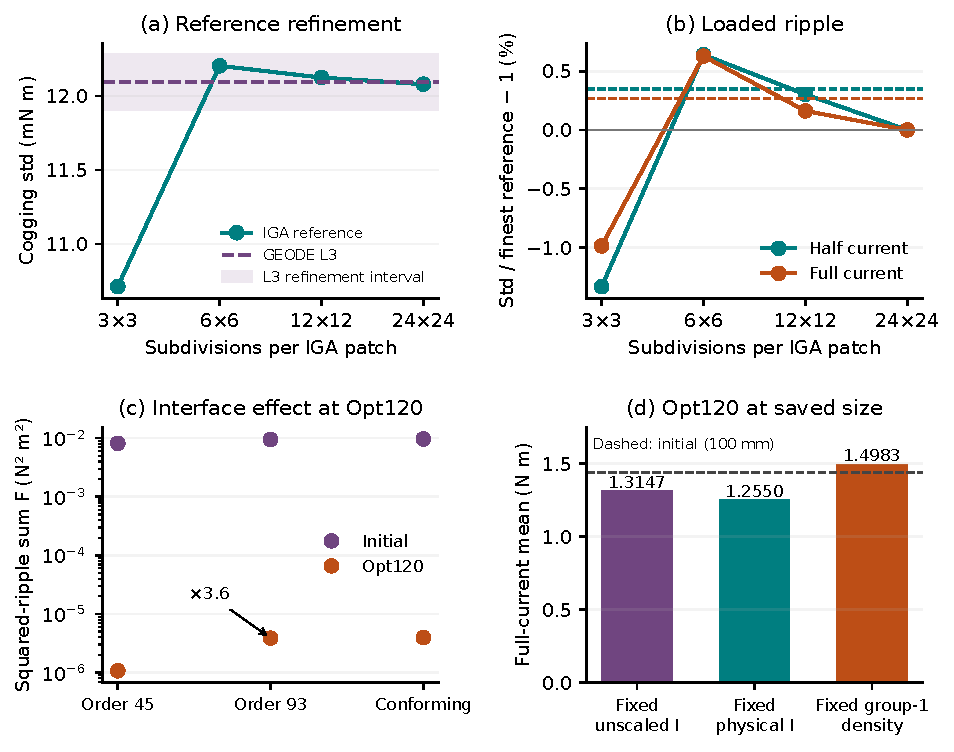
\includegraphics[width=\linewidth]{figures/refined-validation.pdf}
\caption{Reference and candidate validation from raw torque records.
(a) Independent IGA reference cogging refinement at order 45; the dashed
line is GEODE L3 and its shaded band uses Eq.~\eqref{eq:band}.
(b) Loaded standard deviation relative to the finest
reference at each current; circles are IGA, horizontal lines are GEODE L3.
The finest IGA point is zero by construction.
Panels (a,b) use the initial geometry and 20 angles; GEODE uses Arkkio,
with coupling torque checked separately. (c) Initial and Opt120 squared
ripple sums at L3 on fresh meshes and 20 angles, under fixed unscaled
current. Harmonic values use coupling torque; conforming values use
outer-band Arkkio. (d) Full-current mean at order 45 for Opt120 under
three current rules at its saved size (Appendix~\ref{sec:opt120-policy});
the dashed line is the initial mean at the initial size. All candidate
values use coupling torque.}\label{fig:validation}
\end{figure}

This agreement still concerns finite discretizations. The last cogging
increments approximately halve; extending that trend would put a limit
near 0.0120\,N\,m, an estimate without a bound. The last two half-current
standard-deviation increments are both about $-0.3\%$ and do not shrink;
we therefore leave its remaining error unestimated. The 0.10\% cogging
agreement is a comparison of finite-resolution values, not an accuracy
bound; neither refinement sequence is fully converged.
Tightening the reference Newton stopping threshold from $10^{-6}$ to
$10^{-14}$ changes the checked cogging torques by at most
$4.4\times10^{-8}$\,N\,m. GEODE retains straight-sided geometry, and the
high-field extrapolation of the iron law has not been varied in a paired
torque experiment. Neither cross-code agreement nor refinement proves
physical accuracy for the machine.

\subsection{The saved optimized design}\label{sec:opt120}
The saved reference design at iteration 120, denoted Opt120, includes
12 scalar parameters and ten grouped surface-control offsets. We evaluate
its full exported geometry on freshly generated meshes; simply moving
the finest initial mesh produces four inverted triangles. Its inner
air-gap band no longer has the annular area assumed by the full-band
Arkkio functional, so harmonic results here use coupling torque.
Conforming results use only outer-band Arkkio on the fresh exported mesh.
On the same L3, order-45 Opt120 field at full current, the outer-band and
coupling estimates differ by about $1.3\times10^{-4}$\,N\,m in mean and
$1.1\times10^{-5}$\,N\,m in standard deviation. This paired check supports
the estimator substitution at this resolution.
This estimator restriction is specific to these geometries; it does not
validate outer-band Arkkio on arbitrary moved meshes or stator offsets.

With the evaluation current held fixed in the unscaled geometry, raising
the transmitted order from 45 to 93 multiplies Opt120's $F$ by 3.6, from
$1.07\times10^{-6}$ to $3.86\times10^{-6}\,\mathrm{N^2\,m^2}$
(Fig.~\ref{fig:validation}c). The initial design's
$F$ rises by 16\%. Its ratio to Opt120 is consequently 7,631 at order 45,
2,454 at order 93 and 2,444 for conforming coupling. The full-current
Opt120 standard deviation rises from 0.00066 to 0.00164\,N\,m.
The large ripple reduction survives these checks, but its magnitude
depends strongly on the interface model: the order-93 change is about 96
times the last spatial-refinement increment of $F$
(Appendix~\ref{sec:opt120-policy}).

A possible explanation is that optimization against order 45 favors
cancellation within that truncated model. This is a conjecture, not an
ablation result: increasing the order raises full-current ripple but
lowers Opt120 cogging standard deviation from 0.00061 to 0.00035\,N\,m.
Section~\ref{sec:exp2-refinement} reports the corresponding training-to-validation
ratios at the designs selected in the optimization study.
Opt120 is also outside the fixed-size, fixed-physical-current problem of
Section~\ref{sec:optimization}: it shortens the stack from 100 to 80\,mm and
scales the radius by 1.0477, so its mean torque must be compared with the
initial motor only after both size factors and the current rule are fixed.
Appendix~\ref{sec:opt120-policy} gives those normalizations, a reproduction
comparison at the saved reference current, and the effect of angular
sampling at this low ripple.

\section{Design-gradient verification}\label{sec:gradients}
\subsection{Differentiated model and excitation policy}
For a design vector $p$, the converged state $z$ contains the reduced
potential and, for harmonic coupling, its multipliers. Writing the full
constrained residual as $R(z,p)=0$, the discrete adjoint is
\begin{equation}
 R_z^T\psi=F_z^T,\qquad
 \frac{\dd F}{\dd p}=F_p-\psi^T R_p.
 \label{eq:adjoint}
\end{equation}
We differentiate mesh coordinates, element terms, magnet sources, current
loads, harmonic constraints and the torque functional. The explicit
coordinate derivative of Arkkio is included for conforming coupling.
Fixed-topology mesh motion $X(p)$ supplies the chain rule
$\dd F/\dd p_k=\langle\dd F/\dd X,\partial X/\partial p_k\rangle$
for geometric parameters, with direct terms added where needed.

The 12 parameters comprise nine geometric lengths (MAG, MH, MW,
SW1--SW4, SD1 and Sr1), axial length, operating angle and radial scale.
The two designs are the initial parameters and an interior point halfway
toward the saved optimized scalar parameters
(Appendix~\ref{sec:parameters}). This verifies a local scalar
parametrization. The reference's optimized geometry also uses grouped
surface-control displacements; reproducing its 12 scalar values alone
does not reproduce that geometry. The gradients that the optimizers of
Section~\ref{sec:optimization} used, including the grouped offsets of space B
and its mesh-motion map, are checked separately there.

In this scalar derivative study, fixed current means fixed peak current
in the unscaled geometry, so
$J_g=12s_g I_q/|\Omega_g(X)|$ changes when a slot changes area.
For comparison we implement the reference optimizer's rule, denoted
\emph{fixed group-1 density}: $I_*\propto |\Omega_1(X)|s$, where $s$ is
radial scale, with the proportionality constant fixed at the initial
design. The unscaled geometry is evaluated and torque is multiplied by
$s^2$, following the reference. Both rules agree at the initial geometry
but have different derivatives. Group-2 density is not held fixed because
the ratio of the two winding areas can change. At L1 (harmonic coupling,
coupling torque, full current), the mean-torque derivative with respect to SW1 is
$+1.68$\,N\,m/m under fixed current and $-220.85$\,N\,m/m under fixed
group-1 density (Fig.~\ref{fig:gradients}). SW1 is the stator-tooth-width
parameter. The sign change comes from the additional winding-area/current
term: a wider tooth narrows the slot and lowers current under fixed
group-1 density. At this state the policy changes seven of the ten
geometric/scale derivatives and reverses the mean-torque signs for SW1,
SW4 and SD1. Rotor parameters MAG, MH and MW leave winding area unchanged
and therefore give identical derivatives under the two rules. The
fixed-size problem of Section~\ref{sec:optimization} sets radial scale to
one, making fixed physical and unscaled current coincide, and holds that
fixed physical current for every method.

\subsection{Finite differences and Taylor remainders}
The derivative objectives are mean torque and population standard
deviation on the ten even mechanical angles, matching the reference's
optimization grid. Central differences move the same mesh at $p\pm h e_k$;
step sweeps separate truncation from floating-point and nonlinear-solve
error. We also check the first-order remainder
$|F(p+h e_k)-F(p)-h\,\dd F/\dd p_k|$ for quadratic decay.

Across initial and perturbed designs, L0--L2 and the recorded loaded
current/rule subsets, there are 800 objective--parameter records. They pool
harmonic/coupling-torque and conforming/Arkkio evaluations. The fixed-density
MAG, MH and MW records repeat 96 fixed-current comparisons byte-for-byte,
leaving 704 distinct comparisons. Of these, 688 have a best-step relative
error at most $2.8\times10^{-7}$; the maximum is $1.07\times10^{-5}$ for
a small Sr1 ripple derivative. This is a best-step verification statistic,
not the accuracy of a finite-difference step chosen in advance.
Figure~\ref{fig:gradients} includes the 704 distinct cases and an explicit
Taylor sweep. The artifact retains every step, rejected displacement and
relative error. The recorded subsets do not form a full factorial study.

\begin{figure}[!t]\centering
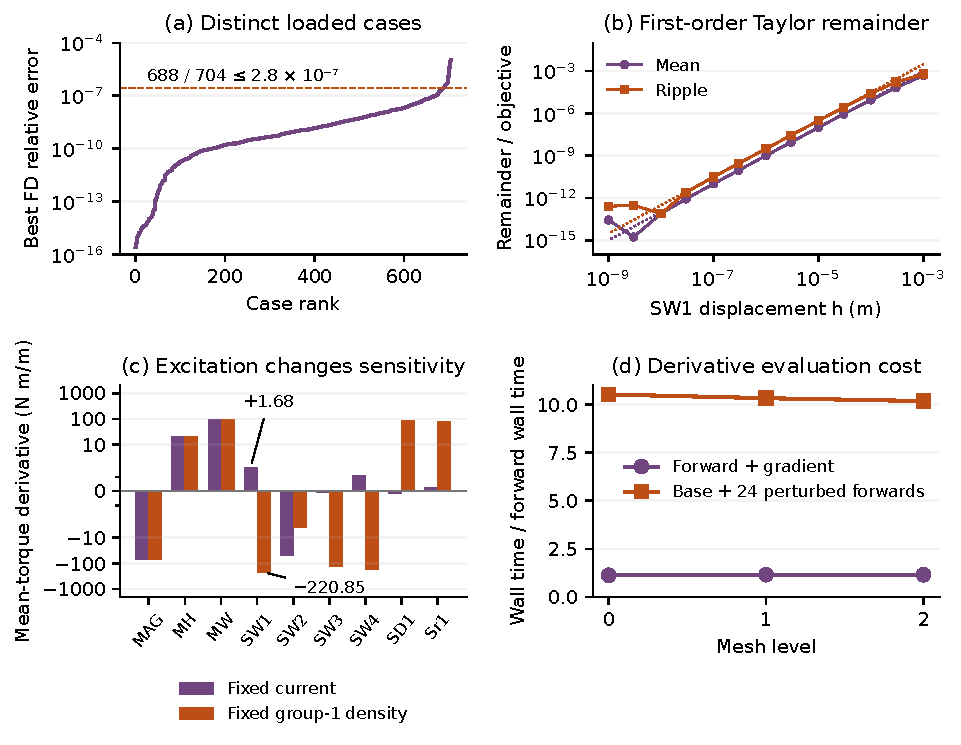
\includegraphics[width=\linewidth]{figures/design-gradients.pdf}
\caption{Discrete gradient evidence. (a) The 704 distinct loaded best-step
finite-difference errors, sorted, pooling harmonic/coupling-torque and
conforming/Arkkio objective--parameter cases. (b) SW1 Taylor remainders at L1, initial design,
full current, harmonic coupling and coupling torque, fixed current; the
plotted remainders are divided by $|F(p)|$, and dotted $h^2$ guides are anchored at $h=10^{-5}$\,m. (c) Mean-torque sensitivities for the nine geometric
parameters under two current rules at that same state; the vertical axis
is symmetric-log, linear within $\pm2$\,N\,m/m. (d) Recorded cost
ratios for harmonic coupling at tolerance $10^{-14}$; gradients include
the forward evaluation, and FD includes its shared base forward.
L0/L1 use medians of three runs, L2 a single run; the seconds are in
Appendix~\ref{sec:cost}.
These timing data were collected under uncontrolled host load.}
\label{fig:gradients}\end{figure}

After removing duplicates and the analytic axial-length and radial-scale
cases, 530 of 592 loaded comparisons have an anchored quadratic-remainder
window spanning at least four decades in step size; 388 span at least five.
The window is the contiguous run where remainder/$h^2$ stays within a
factor of two of its value at $h=10^{-5}$\,m (or $10^{-2}$ degrees for
operating angle). Smaller gradients reach round-off sooner. An anchored-window diagnostic fails for the initial-design, full-current
conforming/fixed-density SW1 ripple cases at L0 and L1: at L0 the
remainder changes sign near the anchor, whereas at L1 remainder/$h^2$ is
still drifting there. Their widest quadratic windows span two decades. The nearly cancelling
zero-current mean is a weaker check: its best relative errors reach
$7.0\times10^{-4}$. Cogging standard-deviation errors are at most
$8.9\times10^{-7}$. Thus the loaded agreement does not describe every
zero-current derivative. Discrete derivative accuracy also does not imply
mesh convergence (Appendix~\ref{sec:cost}).

\subsection{Model dependence of verified sensitivities}
The two model--estimator pairs give different ripple sensitivities even
at the same design (Fig.~\ref{fig:modelgradients} in Appendix~\ref{sec:cost}). At L2 and full fixed
current, the MAG ripple derivative is 1.28\,N\,m/m for harmonic/coupling
torque versus 1.94 for conforming/Arkkio at the initial design. At the
perturbed design the values are 0.75 and 1.87\,N\,m/m. These differences
persist under mesh refinement. At L3 the MAG pairs are 1.22 versus 1.87
at the initial design and 0.57 versus 1.67\,N\,m/m at the perturbed design.
In particular, the latter harmonic component changes appreciably even
though the box-scaled vector changes by only 1.19\% of its L2 norm;
the norm itself decreases by 0.19\%. Mean-torque
sensitivities agree more closely in the box-scaled comparison: the
Euclidean norm of the vector difference, divided by the conforming vector
norm, is 0.58\% and 0.66\% for the mean at the initial and perturbed
designs, versus 6.7\% and 10.2\% for ripple. The norm weights the largest
components most heavily: the initial SW2 and SW3 mean components differ
by 6.5\% and 16.5\% relative to conforming values.
At L3, the ripple gaps remain 6.58\% and 10.25\%, while each model
changes by 0.46--1.19\% from L2 to L3. The mean gaps fall to 0.16\%
and 0.26\%; the conforming model itself changes by 0.52--0.54\%.
The L2 mean gap is therefore comparable to spatial refinement, whereas
the ripple gap persists beyond the measured refinement increments. Because the
estimator changes with the model, this experiment measures their combined
effect; it does not isolate an interface-only derivative error or establish
which gradient is closer to the physical machine.

\subsection{Recorded derivative cost}
On one loaded host, across L0--L2, both couplings and tolerances $10^{-8}$
and $10^{-14}$, the full gradient of both aggregate objectives with respect
to all 12 parameters costs 1.13--1.20 forwards, whereas central differences
cost 8.2--10.5 including the shared base solve (Fig.~\ref{fig:gradients}d;
Appendix~\ref{sec:cost} gives the protocol and seconds).

\section{Discussion and limitations}
Within its scope, the optimization study answers the question the
derivative checks leave open. Across five paired starts, two design spaces
and two training resolutions, wherever both reach a common validated target
from the same start, the adjoint-driven SLSQP gets there sooner than COBYQA
at matched resolution. The validate-every-incumbent rule makes about half
of the charged time validation, which compresses the same-resolution
ratios; it also produces most of A's lead over the coarse derivative-free
competitor D in space A, where the non-validation time of the two is
nearly equal. In space B, A's lead over D survives the decomposition. The
ratios are not population estimates for arbitrary starts. The
finite-difference ablation separates gradient access from search strategy:
with SLSQP fixed, the adjoint is 2.47 and 4.11 times faster in the two
spaces, and set against the main study's B/A ratios this leaves factors of
roughly 1.2--1.3 and 1.9--2.0 for the optimizer. These shares are
approximate, because the two sessions ran separately with different time
units, and the ablation is post hoc.

Population methods such as CMA-ES, multi-start strategies and other
surrogates remain untested. Method C was run with the preregistered
settings of Appendix~\ref{sec:settings} and was not tuned; its low
attainment bounds this configuration, not radial-basis surrogates in
general. No reduced physical model, such as a magnetic equivalent circuit
or a waveform model, was compared: D is a coarse finite-element model, not
such a baseline. The linear slotless screening control in
Appendix~\ref{sec:slotless} admits a three-coefficient angular fit at one
geometry; that does not establish generalization across shapes, but it
cautions against inferring an optimization advantage from parameter count
or adjoint cost alone. In space A, every method's best
design sits on the active mean-torque floor, and four of the five reach
the same $0.043F_0$ (C reaches $0.049F_0$). Within this budget and these
methods, the parameterization and constraint, more than the choice among
A, B, D and E, set the attainable ripple there. Space B's lower ripple
combines ten extra offsets with a different mesh-motion map, and part of
it does not carry over to the held-out currents.

The forward model is two-dimensional and magnetostatic. It does not evaluate
thermal behavior, demagnetization, fatigue, end effects, losses or a
complete efficiency map. The comparison uses published computational
artifacts, with no new measurements on a physical motor. The interface
study shows that truncation changes the objective even as spatial error
decreases, and the paired gradient comparison shows changed ripple
sensitivities despite small discrete derivative errors. Local derivative
tests at an interior scalar design do not validate an entire optimization
trajectory. The reference refinement is at the initial design. Denser and
shifted angle grids and additional currents are checked for Opt120 and for
the selected optimization designs; the reference refinement itself was not
repeated at those designs.

\section{Conclusion}
Before trusting a motor gradient, check what it differentiates: here
raising the interface order multiplies the saved optimized design's ripple
objective by 3.6, about 96 times its last spatial-refinement increment, and
the excitation rule reverses mean-torque sensitivities. Judged on a common
validation model stronger than any training model, SLSQP with adjoint
gradients reached each target sooner than COBYQA at the same training
resolution in every comparison where both succeeded, over five starts in
two fixed-size design spaces, and its crossings survived refinement.
Validating incumbents took about half of the charged time, and a coarse
training mesh, which does not make validation cheaper, gained little and
lost reliability. With the optimizer held fixed, finite differences in
place of the adjoint slowed SLSQP by a factor of 2.5 with eight parameters
and 4.1 with 18, so most of the advantage over derivative-free search came
from the gradients and the rest from the optimizer. Whether the advantage holds for other motor problems, other
parameterizations and reduced physical models remains to be tested.

\section*{Code and data availability}
The original forward and gradient evidence is fixed at GEODE commit
\href{https://github.com/rjwalters/geode-fem/tree/910593bad6f64f9f01671c2632b57034e72b9c61}{\texttt{910593ba}}.
The repository contains the
\href{https://github.com/rjwalters/geode-fem/tree/910593bad6f64f9f01671c2632b57034e72b9c61/benchmarks/motor_reference/forward_harmonic}{raw motor runs and analysis},
\href{https://github.com/rjwalters/geode-fem/tree/910593bad6f64f9f01671c2632b57034e72b9c61/benchmarks/motor_reference/geometry}{geometry and mesh-generation scripts},
\href{https://github.com/rjwalters/geode-fem/tree/910593bad6f64f9f01671c2632b57034e72b9c61/benchmarks/motor_shape_gradient/design}{design-gradient sweeps and timing records},
and \href{https://github.com/rjwalters/geode-fem/tree/910593bad6f64f9f01671c2632b57034e72b9c61/benchmarks/motor_nonlinear_m1}{solver verification logs}.
Candidate-validation records are pinned at
\href{https://github.com/rjwalters/geode-fem/tree/224332c526be1191183af82b610973c7778de720/benchmarks/motor_validation}{\texttt{224332c5}},
and independent reference reruns at
\href{https://github.com/rjwalters/geode-fem/tree/8acd21ecf85d89fe077275a3c04ca70b53963d43/benchmarks/motor_reference/reference_refinement}{\texttt{8acd21ec}}.
Reference data are extracted from the authors'
\href{https://github.com/MichaelWiesheu/ICEMsnapshot/tree/b145aaf4ab1a6424828bc941eaf172f48fa0d458}{ICEM snapshot at \texttt{b145aaf4}},
a later repository revision rather than a claim to the original conference
release. Source hashes, extraction checks and the upstream GPL-3.0-or-later license
are retained. Recomputing the physical study requires the separately
documented mesh and solver commands; the benchmark READMEs record the
GEODE-side Gmsh and Rust toolchain versions.
The matched optimization study (Section~\ref{sec:optimization}) follows the
optimization harness at
\href{https://github.com/rjwalters/geode-fem/tree/9486a9da58beeca91968d4d3608f06b998abff45/benchmarks/motor_optimization}{\texttt{9486a9da}},
the source of the study's evaluator, and its
\href{https://github.com/rjwalters/geode-fem/tree/9486a9da58beeca91968d4d3608f06b998abff45/benchmarks/motor_optimization/runs}{training-gradient finite-difference records};
the final-refinement program is at
\href{https://github.com/rjwalters/geode-fem/tree/3e4ee0c63a86dbf014a76c9faf04dd962da16911/crates/geode-core/examples/icem_final_refinement.rs}{\texttt{3e4ee0c6}}.
The paper package is the directory
\texttt{papers/motor-gradient-optimization/motor-gradient-optimization.11}
of the \href{https://github.com/rjwalters/geode-fem}{GEODE repository}. It
contains a manifest of every copied input with its source commit and
SHA-256, the figure inputs and regeneration scripts (rebuilding the figures
does not require rerunning FEM), two standard-library verifiers that
recompute the reported numbers from those inputs, the per-run validation
histories and ledger charges, the 213 final-check results, copies of the
training-gradient checks, and the study's SHA-256 inventory of all 5,453
output files. The inventory was taken when the session finished; its
existence by 2026-10-20 03:50~UTC is timestamped (RFC~3161 and
OpenTimestamps), and each extracted run and session record is bound to it
by hash. The session, calibration and anchor-recomputation records are
included, as is an export of the governing preregistration comments taken
on 2026-10-18 at 09:34~UTC, before the main session began at 18:16~UTC.
For the post-hoc ablation, the package holds the 40 run extracts, the
setup records, the ablation's SHA-256 inventory of 2,118 files with its
RFC~3161 and OpenTimestamps records, the final-check results, an export of
its protocol and a third verifier; the ablation's evaluator source is
\href{https://github.com/rjwalters/geode-fem/tree/5cc86ad81aeea4847a2608fcafde22a1bbfb6990/benchmarks/motor_optimization}{\texttt{5cc86ad8}}.

\appendix
\section{Field model details}\label{sec:fieldmodel}
\subsection{Nonlinear field equation}
The two-dimensional magnetic vector potential $A=A_z$ determines the
flux density $\mathbf B=(\partial_y A,-\partial_x A)$. Iron is described
by an isotropic reluctivity $\nu(|\mathbf B|^2)$, where reluctivity is
the inverse of permeability. For a test function $v$ that satisfies the
homogeneous constraints, the weak equation is
\begin{equation}
 \int_\Omega \nu(|\nabla A|^2)\nabla A\cdot\nabla v\dd\Omega
 =\int_\Omega J_z v\dd\Omega
  +\int_{\Omega_m}\mathbf M\cdot(\partial_y v,-\partial_x v)\dd\Omega.
 \label{eq:weak}
\end{equation}
Here $\mathbf M$ denotes the permanent-magnet source in
$\mathbf H=\nu\mathbf B-\mathbf M$. In the magnet,
$\mu_r=1.05$ and $B_r=1.4$\,T, so its source magnitude is
$H_c=B_r/(\mu_0\mu_r)$, not $B_r/\mu_0$. Its direction is $\pi/2$
in the rotor frame and rotates with the rotor. Air and windings have
$\mu_r=1$. The inner and outer circular boundaries have $A=0$.

We use continuous piecewise-linear triangles. With nodal vector $u$,
element gradients $g_i=\nabla\varphi_i$, $G=\nabla A$ and $s=G\cdot G$,
the residual derivative on one element is
\begin{equation}
 K^e_{ij}=|\Omega_e|\left[\nu(s)g_i\cdot g_j
       +2\nu'(s)(g_i\cdot G)(g_j\cdot G)\right].
 \label{eq:tangent}
\end{equation}
The second term is required when the material changes with field strength.
Newton steps use this consistent tangent, with damping and a stopping
reference independent of the initial guess. Constant potential offsets,
where allowed by the boundary conditions, do not change that reference.
The solver reports whether it stopped at the requested tolerance or an
estimated floating-point floor. All 500 baseline and sensitivity solves, and all 1,140
additional harmonic-coupling solves, stopped at the requested tolerance.

The iron law uses 47 tabulated M27 $B$--$H$ points from 0 to 2.30\,T.
Monotonicity is imposed on $H(B)$, not on $\nu(B^2)=H(B)/B$.
The tabulated $H/B$ is non-monotone up to about 0.75\,T.
The two material tangent eigenvalues must satisfy
\begin{equation}
 \nu>0,\qquad \nu+2s\nu'=\frac{\dd H}{\dd B}>0.
\end{equation}
The GEODE and reference interpolants agree to round-off between 0.05 and
2.25\,T. GEODE uses an odd cubic near zero and a continuous slope into the
vacuum-slope tail above 2.30\,T. The reference uses a low-field clamp and
a different last-knot slope. The maximum relative difference in
reluctivity near zero is 6.66\%; the last segment differs in $H$ by at
most $2.17\times10^{-4}$ relatively. Appendix~\ref{sec:controls} tests the
torque effect of the low-field difference.

\subsection{Rotation, coupling and torque}
At the modeled angles, the two circular traces have matching nodes after
rotation. Our conforming interface identifies their potentials, including
the antiperiodic sign on sector wrap-around. Writing the full nodal vector
as $u=P\hat u+u_D$, the reduced residual and tangent are
$\hat R=P^T R(P\hat u+u_D)$ and $\hat K=P^T K P$.
The rotor geometry and magnet source rotate together; currents use the
same mechanical angle in Eq.~\eqref{eq:current}.

We average Maxwell stress over the air gap using the Arkkio expression
\citep{arkkio1987}
\begin{equation}
 T(\beta)=\frac{L}{\mu_0(r_2-r_1)}
  \int_{\Omega_{\rm gap}}r B_r B_\theta\dd\Omega,
 \qquad(r_1,r_2)=(44,45)\ {\rm mm}.
 \label{eq:torque}
\end{equation}
Positive torque acts counter-clockwise on the rotor. All torques in this
paper include axial length and refer to the modeled sector. We apply no
factor of six when comparing with the saved reference arrays, despite a
per-length label appearing in the reference evaluation plots.

The alternative harmonic model imposes
\begin{equation}
 \int_{\Gamma_c}(A_s-A_r)e_n\dd\Gamma=0,\qquad
 e_n\in\{\sin(n\theta),\cos(n\theta)\},\quad n=3,9,\ldots,N_h,
\end{equation}
with maximum order $N_h=45$ unless stated otherwise. The 16 order-45
constraints match the reference's eight orders. Rotor and stator
retain distinct trace unknowns. With constraint matrix $C$, Lagrange
multipliers $\eta$ and reduced potential $\hat u$, Newton's method uses
the saddle tangent
\begin{equation}
 \begin{bmatrix}K&C\\ C^T&0\end{bmatrix}.
\end{equation}
The trace moments use the exact Fourier integrals of the piecewise-linear
hats. Rotation enters their centers; the constrained energy derivative gives
\begin{equation}
 T_c=-L\eta^T\frac{\partial(C^T\hat u)}{\partial\beta},
 \label{eq:couplingtorque}
\end{equation}
with the state held fixed in the partial derivative, consistent with
\citet{egger2022torque}. Forward comparisons use Arkkio for both GEODE
couplings to isolate the interface change; coupling torque is a separate
check. The derivative study uses coupling torque for the harmonic model
and Arkkio for the conforming model. The two objectives and their gradients
are consequently comparisons of those specified model--estimator pairs.
The optimization study trains on order-45 coupling torque and validates on
order 93.

The main harmonic runs retain antiperiodic trace-end pairing. An additional
set frees those ends, matching the reference's treatment. The full-order
identity check is summarized in Section~\ref{sec:model}.

\subsection{Implementation checks}
The nonlinear implementation is checked against linear assembly, residual
finite differences, a manufactured solution and a saturated annulus with
an independent radial field relation. Sector tests compare the
constrained solution with a full-machine solve, check the reduced tangent
by finite differences, and exercise positive, negative and wrapped rotation
steps. Clockwise and counter-clockwise triangle orderings give equivalent
magnet sources and fields. The motor regression also detects changes in
magnet strength, magnet direction, phase ordering and rotation direction.
The verification records are linked in the data-availability section.

\section{Optimizer and search settings}\label{sec:settings}
Table~\ref{tab:settings} lists the settings a replication needs beyond
Section~\ref{sec:optimization}; the pinned harness documents them in full.
All methods work in the unit box $u\in[0,1]^n$ of the free coordinates,
minimize $F_{\mathrm{train}}/F_{\mathrm{train}}(\theta_0)$ and impose the
mean floor as $\mu_{\mathrm{train}}/\mu_{\mathrm{train}}(\theta_0)-1.0025\geq0$.
No method validates its start point, and a point validated once is not
validated again.

\begin{table}[H]\centering\small
\caption{Optimizer settings. $n$ is the number of free coordinates (8 or
18), $x_v$ the last admissible evaluated point and $x$ a refused request.}
\label{tab:settings}
\begin{tabular}{>{\raggedright\arraybackslash}p{.11\linewidth}>{\raggedright\arraybackslash}p{.83\linewidth}}\toprule
Method & Settings\\\midrule
A, E & SciPy SLSQP, \texttt{ftol} $10^{-15}$, \texttt{maxiter} $10^5$. Adjoint gradients of the objective and the mean constraint; analytic Jacobians of the geometry constraints. Safeguard: a refused request (unbuildable, mesh-infeasible or derivative undefined) aborts the current solve; the first admissible point $y_k=x_v+2^{-k}(x-x_v)$, $k=1,\ldots,20$, is restored and SLSQP restarts from it with fresh state, at most 20 times. Validation: each iterate the SLSQP callback reports.\\
B, D & SciPy COBYQA, $2n+1$ initial interpolation points, trust radius $0.1$ to $10^{-6}$, \texttt{maxiter} $=$ \texttt{maxfev} $=10^9$. A refused point returns NaN for objective and mean constraint; geometry constraints keep their values. Validation: the callback's best point whenever it changes, after the initial set.\\
C & Four cubic radial-basis interpolants, $\phi(r)=r^3$ with a linear tail: the three training-current standard deviations, each over $\sqrt{F_{\mathrm{train}}(\theta_0)}$, and the full-current mean, refitted after every evaluation. Initial design: the start and $u_0\pm\Delta_0e_i$, $\Delta_0=0.1$ ($n+1$ points). Subproblem: SLSQP on the surrogate in the box and $\|u-u_k\|_\infty\leq\Delta$, at most 200 iterations. Acceptance: a candidate better than the incumbent, feasible first (lower violation, then lower $F$). On acceptance with $\rho\geq0.75$ and a step of at least $0.9\Delta$, $\Delta\leftarrow\min(2\Delta,0.5)$; on rejection $\Delta\leftarrow\Delta/2$, with a geometry point $u_k\pm\Delta e_j$ after every second rejection. Stop at $\Delta<10^{-6}$. Refused points are skipped and count as rejections. Validation: each acceptance.\\
\bottomrule\end{tabular}
\end{table}

The Latin-hypercube starts \citep{mckay1979comparison} use seeds 1--4;
the computations use NumPy \citep{harris2020array} and SciPy
\citep{virtanen2020scipy}.

\section{Per-start times, ratios and final checks}\label{sec:exp2-times}
\begin{table}[H]\centering\small
\caption{Charged wall-time units to the first attaining validation,
repeat~1. A dash means the target was not attained within 120 units.
$T_{99}$ was attained by no run in space A.}
\label{tab:exp2-time}\begin{tabular}{llrrrrr}\toprule
Space, target & Method & $\theta_0$ & LHS 1 & LHS 2 & LHS 3 & LHS 4\\\midrule
A, $T_{50}$ & A & 2.7 & 2.5 & 2.6 & 2.7 & 5.1\\
 & B & 8.5 & 9.3 & 9.3 & 8.9 & 13.7\\
 & E & 1.9 & 1.8 & 1.0 & 3.0 & ---\\
 & D & 3.1 & 5.3 & 7.3 & 4.8 & 8.8\\
 & C & 10.0 & 9.8 & 4.1 & 10.6 & ---\\
\addlinespace
A, $T_{90}$ & A & 2.7 & 2.5 & 7.4 & 6.4 & 8.8\\
 & B & 8.5 & 9.3 & 13.3 & 15.4 & 49.3\\
 & E & 1.9 & 1.8 & 4.5 & 3.0 & ---\\
 & D & 4.6 & 5.3 & 7.3 & 9.4 & 21.9\\
 & C & 16.9 & 9.8 & --- & --- & ---\\
\addlinespace
B, $T_{50}$ & A & 1.6 & 1.7 & 3.0 & 4.8 & 1.6\\
 & B & 12.2 & 13.1 & 13.5 & 21.5 & 15.7\\
 & E & 1.0 & 1.1 & 1.1 & 4.4 & 1.2\\
 & D & 4.1 & 6.9 & 5.2 & 11.9 & 8.4\\
 & C & 7.3 & 8.4 & 7.3 & 12.1 & 8.9\\
\addlinespace
B, $T_{90}$ & A & 3.1 & 5.4 & 3.0 & 12.0 & 1.6\\
 & B & 14.4 & 13.1 & 13.5 & 36.6 & 35.3\\
 & E & 2.0 & --- & 2.8 & 10.9 & 1.2\\
 & D & 5.9 & 8.1 & 5.2 & 15.9 & 14.3\\
 & C & 8.4 & 8.4 & 10.3 & --- & 14.6\\
\addlinespace
B, $T_{99}$ & A & 5.4 & 6.6 & 9.1 & 13.1 & 13.4\\
 & B & 90.4 & 59.1 & 48.6 & --- & 62.3\\
 & E & 3.9 & --- & 6.5 & 10.9 & 8.3\\
 & D & 43.0 & 14.1 & 36.0 & 83.3 & 47.8\\
 & C & --- & --- & --- & --- & 25.9\\
\bottomrule\end{tabular}

\end{table}

\begin{table}[H]\centering\small
\caption{Paired per-start time ratios (repeat~1). B/A and D/E vary the
optimizer at fixed resolution; E/A and D/B vary the resolution; D/A
compares A with the coarse derivative-free competitor. Ratios above one
favor the denominator. Geometric means use the finite pairs only, so the
D/E and E/A means omit the starts where E failed to attain the target.}
\label{tab:exp2-ratios}\begin{tabular}{llrrl}\toprule
Space, target & Ratio & Finite pairs & Geometric mean & Per-start ratios\\\midrule
A, $T_{50}$ & B/A & 5 & 3.25 & 3.18, 3.66, 3.63, 3.25, 2.66\\
 & D/E & 4 & 2.75 & 1.60, 2.90, 7.68, 1.61, ---\\
 & E/A & 4 & 0.68 & 0.72, 0.72, 0.37, 1.09, ---\\
 & D/B & 5 & 0.56 & 0.36, 0.57, 0.78, 0.54, 0.64\\
 & D/A & 5 & 1.83 & 1.15, 2.09, 2.85, 1.75, 1.71\\
\addlinespace
A, $T_{90}$ & B/A & 5 & 3.10 & 3.18, 3.66, 1.80, 2.43, 5.61\\
 & D/E & 4 & 2.45 & 2.41, 2.90, 1.61, 3.17, ---\\
 & E/A & 4 & 0.62 & 0.72, 0.72, 0.61, 0.47, ---\\
 & D/B & 5 & 0.54 & 0.54, 0.57, 0.55, 0.61, 0.44\\
 & D/A & 5 & 1.68 & 1.72, 2.09, 0.99, 1.48, 2.49\\
\addlinespace
B, $T_{50}$ & B/A & 5 & 6.49 & 7.76, 7.70, 4.51, 4.46, 9.59\\
 & D/E & 5 & 4.69 & 3.90, 6.14, 4.93, 2.72, 7.09\\
 & E/A & 5 & 0.63 & 0.66, 0.66, 0.35, 0.91, 0.72\\
 & D/B & 5 & 0.46 & 0.33, 0.52, 0.39, 0.56, 0.53\\
 & D/A & 5 & 2.97 & 2.58, 4.04, 1.75, 2.48, 5.09\\
\addlinespace
B, $T_{90}$ & B/A & 5 & 5.06 & 4.64, 2.41, 4.51, 3.05, 21.54\\
 & D/E & 4 & 3.14 & 2.94, ---, 1.86, 1.46, 12.17\\
 & E/A & 4 & 0.79 & 0.65, ---, 0.94, 0.91, 0.72\\
 & D/B & 5 & 0.45 & 0.41, 0.62, 0.39, 0.44, 0.41\\
 & D/A & 5 & 2.25 & 1.91, 1.50, 1.75, 1.33, 8.74\\
\addlinespace
B, $T_{99}$ & B/A & 4 & 7.79 & 16.65, 8.92, 5.33, ---, 4.65\\
 & D/E & 4 & 7.20 & 11.05, ---, 5.50, 7.65, 5.79\\
 & E/A & 4 & 0.72 & 0.72, ---, 0.72, 0.83, 0.61\\
 & D/B & 4 & 0.50 & 0.48, 0.24, 0.74, ---, 0.77\\
 & D/A & 5 & 4.32 & 7.91, 2.12, 3.94, 6.36, 3.56\\
\bottomrule\end{tabular}

\end{table}

\begin{table}[H]\centering\scriptsize
\caption{Final checks of the selected designs. ``best'' marks a method's
representative; ``A $T_{90}$'' marks the earliest repeat-1 crossing of that
target by that method. The L2 column is the primary check on the
refinement host. L3 and conforming changes are in percent; the 40-angle,
tight and shifted changes are relative, in units of $10^{-4}$. ``held-out'' is the objective at currents $0.25$ and
$0.75$ relative to $\theta_0$'s at the same currents. A dash means the
conforming check does not apply because stator offsets are nonzero.}
\label{tab:exp2-refinement}\begin{tabular}{lrrrrrrr}\toprule
Design & $F_{\mathrm{L2}}/F_0$ & L3 & g40 & tight & shifted & conf. & held-out\\
 & & (\%) & ($10^{-4}$) & ($10^{-4}$) & ($10^{-4}$) & (\%) & \\\midrule
\multicolumn{8}{l}{\emph{Space A}}\\
$\theta_0$ & 1.0000 & $-1.3$ & $0.0$ & $0.0$ & $+0.1$ & $+2.1$ & 1.0000\\
best A & 0.0432 & $-0.4$ & $0.0$ & $0.0$ & $+0.1$ & $+4.4$ & 0.0472\\
best B & 0.0432 & $-0.5$ & $0.0$ & $0.0$ & $0.0$ & $+4.4$ & 0.0472\\
best C & 0.0489 & $-0.7$ & $+0.2$ & $0.0$ & $+0.5$ & $+4.1$ & 0.0524\\
best D & 0.0432 & $-0.5$ & $0.0$ & $0.0$ & $0.0$ & $+4.4$ & 0.0472\\
best E & 0.0434 & $-0.6$ & $+0.4$ & $0.0$ & $+0.9$ & $+4.4$ & 0.0473\\
A $T_{50}$, A $T_{90}$ & 0.0653 & $-2.9$ & $+0.7$ & $0.0$ & $+1.5$ & $+1.1$ & 0.0686\\
B $T_{50}$, B $T_{90}$ & 0.0881 & $-2.3$ & $+1.3$ & $0.0$ & $+2.6$ & $+3.2$ & 0.0866\\
C $T_{50}$ & 0.1472 & $-4.0$ & $+0.6$ & $0.0$ & $+1.3$ & $+3.3$ & 0.1508\\
C $T_{90}$ & 0.0507 & $-0.9$ & $+0.2$ & $0.0$ & $+0.5$ & $+4.0$ & 0.0543\\
D $T_{50}$ & 0.0920 & $-2.2$ & $+1.5$ & $0.0$ & $+3.0$ & $+3.3$ & 0.0899\\
D $T_{90}$ & 0.0594 & $-2.3$ & $+1.3$ & $0.0$ & $+2.6$ & $+1.6$ & 0.0609\\
E $T_{50}$ & 0.1105 & $-2.0$ & $+0.6$ & $0.0$ & $+1.1$ & $+1.2$ & 0.1104\\
E $T_{90}$ & 0.0660 & $-2.9$ & $+0.7$ & $0.0$ & $+1.5$ & $+1.1$ & 0.0694\\
\multicolumn{8}{l}{\emph{Space B}}\\
$\theta_0$ & 1.0000 & $-1.3$ & $0.0$ & $0.0$ & $+0.1$ & $+2.0$ & 1.0000\\
best A & 0.0053 & $+2.6$ & $+0.4$ & $+0.1$ & $+0.5$ & --- & 0.0066\\
best B, B $T_{99}$ & 0.0085 & $-3.0$ & $-0.4$ & $0.0$ & $-1.2$ & --- & 0.0076\\
best C, C $T_{99}$ & 0.0057 & $-3.7$ & $+2.5$ & $0.0$ & $+5.0$ & --- & 0.0074\\
best D & 0.0044 & $+6.3$ & $+2.6$ & $+0.1$ & $+4.9$ & --- & 0.0076\\
best E & 0.0071 & $+2.6$ & $-1.5$ & $0.0$ & $-3.1$ & --- & 0.0087\\
A $T_{50}$ & 0.1874 & $+0.9$ & $-0.3$ & $0.0$ & $-0.6$ & --- & 0.1538\\
A $T_{90}$ & 0.0255 & $+1.1$ & $-0.1$ & $0.0$ & $-0.2$ & --- & 0.0248\\
A $T_{99}$ & 0.0077 & $+0.4$ & $-0.1$ & $0.0$ & $-0.3$ & --- & 0.0096\\
B $T_{50}$ & 0.1854 & $-1.5$ & $-0.1$ & $0.0$ & $-0.3$ & --- & 0.1907\\
B $T_{90}$ & 0.0523 & $-0.4$ & $-0.2$ & $0.0$ & $-0.4$ & --- & 0.0505\\
C $T_{50}$ & 0.3958 & $-1.4$ & $-0.1$ & $0.0$ & $-0.1$ & --- & 0.3692\\
C $T_{90}$ & 0.0259 & $+0.7$ & $0.0$ & $0.0$ & $0.0$ & --- & 0.0247\\
D $T_{50}$ & 0.1925 & $-1.5$ & $-0.1$ & $0.0$ & $-0.3$ & --- & 0.1971\\
D $T_{90}$ & 0.0393 & $-0.7$ & $+0.6$ & $0.0$ & $+1.2$ & --- & 0.0392\\
D $T_{99}$ & 0.0089 & $+0.4$ & $-0.5$ & $0.0$ & $-1.0$ & --- & 0.0137\\
E $T_{50}$ & 0.1961 & $+0.8$ & $0.0$ & $0.0$ & $0.0$ & --- & 0.1567\\
E $T_{90}$ & 0.0223 & $-2.8$ & $-5.3$ & $0.0$ & $-10.6$ & --- & 0.0144\\
E $T_{99}$ & 0.0081 & $+0.7$ & $+0.2$ & $0.0$ & $+0.4$ & --- & 0.0112\\
\bottomrule\end{tabular}

\end{table}

\paragraph{Training and validation objectives.}
The training model also reads lower than validation. At $\theta_0$, the
order-45 training objective is 0.887 (L1) and 0.894 (L0) of $F_0$. At the
31 selected designs, the ratio of training to validation objective lies
between 0.57 and 1.19 times its $\theta_0$ value. The lowest values belong
to space-B designs near $T_{99}$: E's and A's $T_{99}$ crossings (0.57 and
0.71) and D's best design (0.65); the best space-B designs of B and C are at
0.99 and 1.19. Large reductions therefore often, but not always, come with a
training objective that underestimates validation more than at $\theta_0$.
This is consistent with the cancellation conjecture of
Section~\ref{sec:opt120} but does not establish it.

\paragraph{Ablation session and finite-difference accuracy.}
On the L0 model, F's gradients agree with the adjoint to a max-norm
relative error of $5.1\times10^{-4}$ to $1.9\times10^{-3}$ for $F$ and
$1.0\times10^{-4}$ to $6.7\times10^{-4}$ for the full-current mean, at
$\theta_0$ and an interior point in each space. Single small components are
less accurate, up to $5.7\times10^{-2}$ for SW3 at the space-B interior
point. These errors, at the frozen step, are part of what F is; the frozen
acceptance limits were $5\times10^{-3}$ for the norm and $10^{-1}$ per
component.

The session ran on the same type of host as the main study (c7a.4xlarge,
15 concurrent processes) with a calibrated unit of $66.66\,\mathrm{s}$,
against $70.94\,\mathrm{s}$ in the main session. The anchor recomputation
again agreed within $2.4\times10^{-13}$, no run was host-contaminated, and
the one-minute load peaked at 19.7. A SHA-256 inventory of the 2,118
session files was taken on the host before it stopped and timestamped by
two RFC~3161 authorities; every number below is recomputed from traces
bound to it.

\paragraph{Ablation final checks.}
The final checks confirm F's and A$'$'s selected designs
(Table~\ref{tab:exp2b-refinement}). All 90 checks of the 14 designs
completed. The primary check reproduces the study's $F_{\mathrm{val}}$
within $6.3\times10^{-4}$ relative. L3 changes $F$ by $-2.9\%$ to $+2.6\%$
($-2.9\%$ to $+1.1\%$ at the crossings), the 40-angle, tight and shifted
checks by less than $0.03\%$, and the conforming estimator gives $1.1\%$ to
$4.4\%$ more ripple on the space-A designs. All ten target crossings keep
their target at L3 with at least 15\% margin, and every candidate keeps the
mean floor, the closest by 0.044\%. An independent selection program chose
the same 14 designs, bit for bit.

\begin{table}[H]\centering\small
\caption{Post-hoc ablation (Section~\ref{sec:exp2-fd}): charged time units
to the first attaining validation for A$'$ and F, repeat~1, and their
ratio per start; the last column gives the geometric mean, with repeat~2 in
parentheses. Units are those of the ablation session.}
\label{tab:exp2b-ratios}\begin{tabular}{llrrrrrl}\toprule
Space, target & & $\theta_0$ & LHS 1 & LHS 2 & LHS 3 & LHS 4 & GM (rep.~2)\\\midrule
A, $T_{50}$ & A$'$ & 2.8 & 2.6 & 2.7 & 2.8 & 5.2 & \\
 & F & 6.9 & 6.5 & 6.5 & 6.7 & 12.7 & \\
 & F/A$'$ & 2.45 & 2.45 & 2.39 & 2.43 & 2.43 & 2.43 (2.44)\\
\addlinespace
A, $T_{90}$ & A$'$ & 2.8 & 2.6 & 7.6 & 6.4 & 8.9 & \\
 & F & 6.9 & 6.5 & 18.9 & 16.3 & 21.8 & \\
 & F/A$'$ & 2.45 & 2.45 & 2.50 & 2.52 & 2.45 & 2.47 (2.49)\\
\addlinespace
B, $T_{50}$ & A$'$ & 1.6 & 1.6 & 3.2 & 4.8 & 1.7 & \\
 & F & 6.3 & 5.6 & 11.3 & 17.8 & 5.9 & \\
 & F/A$'$ & 3.91 & 3.59 & 3.58 & 3.69 & 3.60 & 3.67 (3.68)\\
\addlinespace
B, $T_{90}$ & A$'$ & 3.1 & 5.1 & 3.2 & 12.1 & 1.7 & \\
 & F & 12.2 & 20.8 & 11.3 & 49.9 & 5.9 & \\
 & F/A$'$ & 3.92 & 4.09 & 3.58 & 4.14 & 3.60 & 3.86 (3.84)\\
\addlinespace
B, $T_{99}$ & A$'$ & 5.4 & 6.3 & 9.3 & 13.2 & 13.6 & \\
 & F & 23.6 & 24.0 & 38.7 & 54.9 & 55.8 & \\
 & F/A$'$ & 4.33 & 3.84 & 4.14 & 4.17 & 4.10 & 4.11 (4.04)\\
\bottomrule\end{tabular}

\end{table}

\begin{table}[H]\centering\small
\caption{Validation charges in the ablation, repeat~1, as in
Table~\ref{tab:exp2-validation}.}
\label{tab:exp2b-validation}\begin{tabular}{lllllll}\toprule
 & \multicolumn{3}{c}{Space A} & \multicolumn{3}{c}{Space B}\\\cmidrule(lr){2-4}\cmidrule(lr){5-7}
Method & To crossing & Share & Run & To crossing & Share & Run\\\midrule
A$'$ & 2 (2--7) & 0.65 (0.65--0.70) & 0.44--0.70 & 3 (1--10) & 0.61 (0.58--0.68) & 0.64--0.68\\
F & 2 (2--7) & 0.27 (0.26--0.29) & 0.25--0.28 & 3 (1--10) & 0.16 (0.15--0.18) & 0.15--0.18\\
\bottomrule\end{tabular}

\end{table}

\begin{table}[H]\centering\small
\caption{Final checks of the ablation's selected designs, as in
Table~\ref{tab:exp2-refinement}: L2 objective, L3 change, the largest
40-angle, tight or shifted change, and the conforming change where stator
offsets are zero.}
\label{tab:exp2b-refinement}\begin{tabular}{lrrrr}\toprule
Design & $F_{\mathrm{L2}}/F_0$ & L3 (\%) & max g40/tight/shifted ($10^{-4}$) & conf. (\%)\\\midrule
\multicolumn{5}{l}{\emph{Space A}}\\
$\theta_0$ & 1.0000 & $-1.3$ & 0.1 & $+2.1$ \\
A$'$ $T_{50}$, $T_{90}$ & 0.0653 & $-2.9$ & 1.5 & $+1.1$ \\
F $T_{50}$, $T_{90}$ & 0.0653 & $-2.9$ & 1.5 & $+1.1$ \\
best A$'$ & 0.0432 & $-0.4$ & 0.1 & $+4.4$ \\
best F & 0.0432 & $-0.6$ & 0.1 & $+4.2$ \\
\multicolumn{5}{l}{\emph{Space B}}\\
$\theta_0$ & 1.0000 & $-1.3$ & 0.1 & $+2.0$ \\
A$'$ $T_{50}$ & 0.2721 & $-0.6$ & 3.0 & --- \\
A$'$ $T_{90}$ & 0.0255 & $+1.1$ & 0.2 & --- \\
A$'$ $T_{99}$ & 0.0077 & $+0.4$ & 0.3 & --- \\
F $T_{50}$ & 0.2720 & $-0.6$ & 3.0 & --- \\
F $T_{90}$ & 0.0252 & $+1.0$ & 0.6 & --- \\
F $T_{99}$ & 0.0076 & $+0.4$ & 0.3 & --- \\
best A$'$ & 0.0053 & $+2.6$ & 0.5 & --- \\
best F & 0.0054 & $+2.5$ & 0.2 & --- \\
\bottomrule\end{tabular}

\end{table}

\section{Forward-model controls}\label{sec:controls}
\begin{figure}[H]\centering
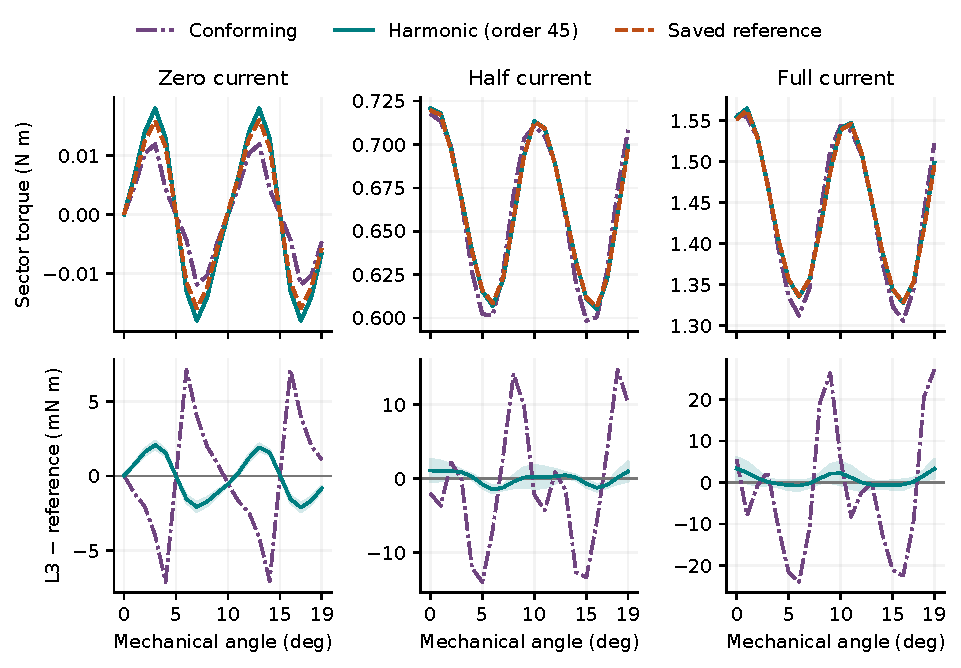
\includegraphics[width=\linewidth]{figures/coupling-waveforms.pdf}
\caption{Top: L3 torque for conforming and order-45 harmonic coupling,
compared with the saved reference. Bottom: each GEODE waveform minus the
reference; shading is the harmonic model's pointwise estimated refinement
interval from Eq.~\eqref{eq:band}. Each residual panel has its own vertical
scale, so compare residual magnitudes by their axis values, not by curve
height. All GEODE curves use Arkkio torque, so the paired difference changes the
coupling while holding the estimator fixed. The saved reference is coarse;
Section~\ref{sec:refinement} reports its refinement.}
\label{fig:waveforms}\end{figure}

The controlled changes in Table~\ref{tab:sensitivity} are too small to
explain the observed waveform gap at the tested settings. The near-zero
material difference has particularly little effect on torque despite its
6.66\% local reluctivity difference. This is a measured sensitivity of
the initial design and does not establish insensitivity after optimization.

\begin{table}[H]\centering\small
\caption{Maximum absolute torque change relative to the baseline at the
same mesh level, using conforming coupling and Arkkio torque. Entries
summarize the recorded angle/current subsets.}
\label{tab:sensitivity}
\begin{tabular}{p{.48\linewidth}ll}\toprule
Change & Levels & Max. $|\Delta T|$ (N\,m)\\\midrule
Reference low-field interpolation and clamp & L2, L3 & $2.1\times10^{-6}$\\
Relative Newton tolerance $10^{-12}$ vs $10^{-8}$ & L2; L3 full current & $7.3\times10^{-8}$\\
Exact winding areas vs mesh areas & L2 & $3.9\times10^{-4}$\\
Inner or outer half of the Arkkio band & L3 & $7.3\times10^{-5}$\\
\bottomrule\end{tabular}
\end{table}

In the recorded estimator study, single-circle Maxwell-stress estimates
vary more with the integration radius than the half-band Arkkio estimates.
The paired coupling-torque and half-band checks of
Section~\ref{sec:forward} avoid selecting a favorable radius. A
post-processing filter of the solved conforming field also gives
non-monotone ripple changes across the tested cuts and currents; it does
not replace a field solve with a truncated interface. The complete filter
results are retained in the accompanying forward-study records.

\section{Opt120: size, current policy and angular sampling}\label{sec:opt120-policy}
Between L2 and L3, changes in
$F$, normalized by L3, reach 1.36\% for the initial design and 2.71\%
for Opt120 across the three models on the exported mesh family; these increments are not error bounds.
For Opt120 at order 45, the successive L1--L2 and L2--L3 increases in $F$
are $3.05\times10^{-8}$ and $2.90\times10^{-8}$\,N$^2$\,m$^2$,
so they barely shrink and do not establish an asymptotic rate. An alternate
freshly constructed mesh family changes by 3.22\% for Opt120 from L2 to L3.
The $2.79\times10^{-6}$\,N$^2$\,m$^2$ interface effect is about
96 times the last export-mesh increment, despite this unresolved remainder.

Current policy changes Opt120's feasibility (Fig.~\ref{fig:validation}d). At L3 and order 45,
the initial full-current mean is 1.4433\,N\,m. Opt120 gives 1.3147\,N\,m
under fixed \emph{unscaled} current, 1.2550\,N\,m under fixed physical
current, and 1.4983\,N\,m under the reference's fixed group-1 density rule.
The first two are 8.9\% and 13.0\% below the initial mean; the density-rule
value is 3.8\% above it. These policy comparisons use the same Opt120
geometry, but comparisons with the initial motor also change size:
Opt120 shortens the stack from 100 to 80\,mm and has radial scale
$s=1.0477$, unscaled outer diameter 130.293\,mm and operating angle
$-11.646^\circ$ (Table~\ref{tab:parameters}). Every Opt120 torque carries
the explicit size factor $s^2L/(0.1\,\mathrm{m})=0.878175$.
Removing both size factors from the fixed-unscaled-current mean gives
1.4971\,N\,m, 3.7\% above the initial mean. Applying the same normalization
to fixed physical current gives 1.4291\,N\,m, 1.0\% below the initial mean;
the density-rule value becomes 1.7061\,N\,m, 18.2\% above it. Normalizing
only length to 100\,mm under fixed unscaled current gives 1.6434\,N\,m
(+13.9\%), retaining the radial factor $s^2=1.098$.
These algebraic normalizations separate the size factors from the current
rule; they are not reoptimized designs. Most of the saved-size deficit
therefore comes from the size factor, although the normalized
fixed-physical-current value remains lower.

A separate reproduction comparison uses the saved reference current at
each design, rather than fixed unscaled current. At Opt120, GEODE's
order-45 full-current mean is 1.4986\,N\,m versus 1.5000\,N\,m in the
saved arrays, but its standard deviation is $3.53\times10^{-4}$ versus
$1.76\times10^{-4}$\,N\,m, a factor of 2.0. The half-current values are
$5.53\times10^{-4}$ and $4.37\times10^{-4}$\,N\,m.
The largest pointwise difference across the two loaded currents is about
$2.1\times10^{-3}$\,N\,m. With this matched current policy and zero-current
values included (zero current is rule-independent and taken from the
fixed-current record), the initial-to-Opt120 objective ratios are 10,170 for
GEODE and 11,982 for the saved reference. The 7,631 ratio of
Section~\ref{sec:opt120} instead holds unscaled current fixed. Reference
refinement was run only at the initial design, so the cause of the Opt120
discrepancy remains unresolved.

Angular sampling becomes more consequential at this low ripple. Relative
to the 40-angle grid, the ten-angle Opt120 objective reads about 1.05\%
high at order 45 and 5.90\% low at order 93 on the fresh L3 mesh; the
conforming value reads 17.1\% low. The accompanying records retain shifted
20-angle grids and withheld currents 0.25 and 0.75. Candidate validation
must check these effects at the candidate, since initial-design agreement
alone would miss them. All 3,240 solve rows in the 18 successful records used for
these candidate comparisons stopped at tolerance.
Figure~\ref{fig:opt-waveforms} shows the full and mean-subtracted waveforms.

\begin{figure}[H]\centering
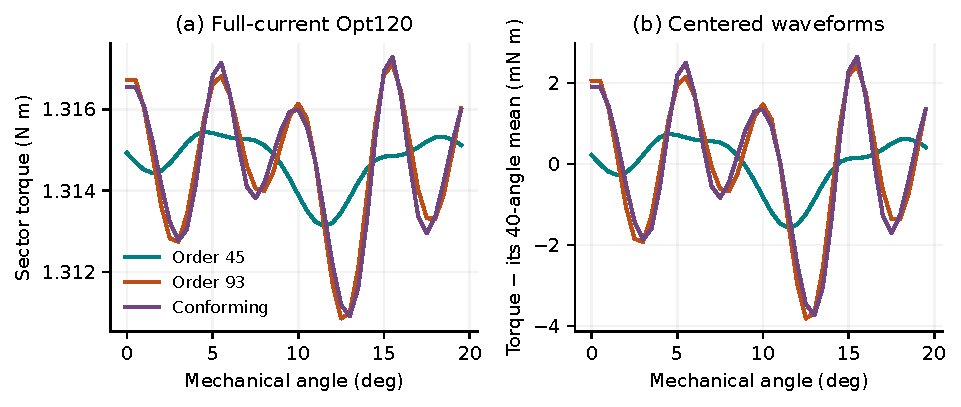
\includegraphics[width=\linewidth]{figures/opt120-waveforms.pdf}
\caption{Opt120 full-current torque on fresh L3 meshes at 40 angles,
with fixed unscaled current. Harmonic orders 45 and 93 use coupling torque;
conforming coupling uses outer-band Arkkio. Left: full torque, retaining
each model's mean. Right: each curve minus its own 40-angle mean.
The interface change mainly alters the resolved ripple.}
\label{fig:opt-waveforms}
\end{figure}

\section{Model-dependent sensitivities and derivative cost}\label{sec:cost}
Discrete derivative accuracy also does not imply mesh convergence. In the
harmonic model, SW3 mean-torque sensitivities change sign between coarse
levels and their increments shrink with refinement; ripple gradients converge
more slowly than most mean gradients. The conforming/Arkkio SW2 mean
sensitivity is non-monotone across L0--L3 ($-46.5$, $-41.3$, $-44.4$,
$-47.2$\,N\,m/m), whereas harmonic/coupling torque approaches $-47.1$
from $-49.8$\,N\,m/m. Fresh-remesh checks of MW, SW1 and SW2 are limited
at small steps by changes in connectivity. The L2 MW mean-derivative fit
has relative gap $2.6\times10^{-6}$, but individual remeshed steps at
$h\geq10^{-4}$\,m scatter by about $6\times10^{-4}$. The largest L2 full-current
remeshed-versus-moved fitted discrepancy is 3.8\% for the SW1 ripple
derivative. These checks support the discrete chain rule while leaving
refinement of candidate designs necessary.

\begin{figure}[H]\centering
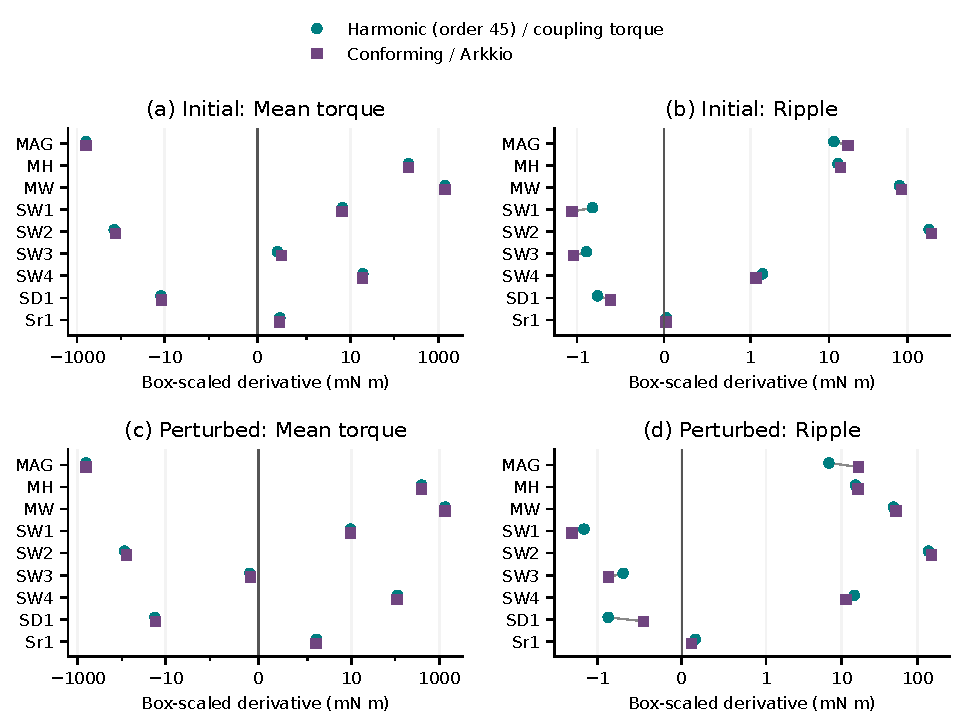
\includegraphics[width=\linewidth]{figures/model-gradients.pdf}
\caption{Full fixed-current sensitivities at L2, scaled by each geometric
parameter's reference box width $w_k$. Top: initial design; bottom:
perturbed design. L3 MAG values and refinement changes are given in the
text. Left: mean torque; right: standard deviation. The plotted
quantity $w_k\partial q/\partial p_k$ is a local sensitivity, not a finite
change across the box. Coupling and torque estimator both differ between
the two series. Gray segments join the two estimates for each parameter. Horizontal axes are symmetric-log, linear within
$\pm1$\,mN\,m. All nine widths, in mm, are 9, 10, 15, 4, 3, 1, 18, 70 and
1.5 in the displayed order.}\label{fig:modelgradients}
\end{figure}


The recorded timings use an Apple M3 Ultra with 28 cores, default solver
threading, and concurrent host load averaging 14--24. The effective thread
count was not pinned. A forward evaluation covers ten angles, starts from
zero, and warm-starts successive angles. The full gradient includes that
forward, ten torque adjoints, mesh derivatives and contractions for all
12 parameters and both aggregate objectives. Central differences use 24
forward sweeps, each warm-started from the base states, at step
$h=10^{-6}$ in each parameter's stored unit (m, degrees or dimensionless
scale), plus the shared base forward for a common starting point. Across
L0--L2, both couplings and tolerances $10^{-8}$ and $10^{-14}$, the full
gradient costs 1.13--1.20 forwards, whereas central differences cost
8.2--10.5 including the shared base solve (Fig.~\ref{fig:gradients}d and
Table~\ref{tab:cost}). Shape-map setup is a separate one-time cost of
these timings; the optimization study charges whole-run wall time, so it is
included there. These derivative timings concern one loaded host and are a
separate workload from the 1,640 forward validation solves of
Section~\ref{sec:forward}.

\begin{table}[H]\centering\small
\caption{Recorded harmonic-model cost at relative tolerance $10^{-14}$,
initial design and full current. Times are seconds for ten-angle sweeps;
FD includes the shared base sweep, and setup is a one-time shape-map cost.}
\label{tab:cost}\begin{tabular}{lrrrr}\toprule
Mesh & Forward & Forward + gradient & Base + FD & Setup\\\midrule
L0 & 0.664 & 0.748 & 6.997 & 0.011 \\
L1 & 3.174 & 3.658 & 32.811 & 0.041 \\
L2 & 12.702 & 14.644 & 129.390 & 0.222 \\
\bottomrule\end{tabular}

\end{table}

\section{Linear slotless screening control}\label{sec:slotless}
The stored slotless model has 24 distinct angles. Fitting
$T(\phi)=c_0+c_1\cos\phi+c_2\sin\phi$, with electrical angle $\phi=p\theta_r$, mechanical rotor angle $\theta_r$
and pole-pair count $p$, on alternate angles and
evaluating on the other twelve gives normalized held-out RMSE
$3.08\times10^{-10}$ and maximum error $6.82\times10^{-10}$, using the
recorded analytic-amplitude normalization. This is a locked-rotor angle sweep,
not synchronous operating ripple. For a fixed linear field operator and
sinusoidal sources, the field lies in a small basis of source responses;
a quadratic torque functional can contain only the corresponding finite
set of harmonics. The particular model needs just the three fitted
coefficients. This is an angular interpolation test at one geometry,
not a shape-gradient test or evidence of generalization across designs.

\section{Design points for derivative checks}\label{sec:parameters}
Table~\ref{tab:parameters} identifies the scalar derivative-study coordinates
and the saved Opt120 coordinates. Values are rounded for display; the accompanying records
retain full precision. The operating angle is stored in degrees and
converted to radians in the current equation. These coordinates describe
the scalar design space; the saved reference optimum additionally contains
surface-control offsets.
\begin{table}[H]\centering\small
\caption{Initial and interior perturbed design points for derivative
checks, alongside Opt120 for the forward validation. Lengths refer to the
unscaled geometry; surface-control offsets are retained in the data.}\label{tab:parameters}
\begin{tabular}{l>{\raggedright\arraybackslash}p{.28\linewidth}lrrr}\toprule
Parameter & Meaning & Unit & Initial & Perturbed & Opt120\\\midrule
MAG & Pole-axis iron depth above magnet & mm & 7.0000 & 6.5506 & 6.1011 \\
MH & Radial magnet height & mm & 7.0000 & 4.8722 & 2.7444 \\
MW & Magnet width & mm & 19.0000 & 19.8670 & 20.7340 \\
SW1 & Stator tooth width & mm & 4.0000 & 4.0309 & 4.0619 \\
SW2 & Slot-opening width & mm & 2.3000 & 1.6500 & 1.0001 \\
SW3 & Slot-opening depth & mm & 1.0000 & 0.7502 & 0.5004 \\
SW4 & Back-iron depth on slot axis & mm & 8.2500 & 6.8418 & 5.4336 \\
SD1 & Stator outer diameter & mm & 135.0000 & 132.6466 & 130.2931 \\
Sr1 & Slot-bottom fillet radius & mm & 1.0000 & 1.4999 & 1.9998 \\
LENGTH & Axial length & mm & 100.0000 & 90.0003 & 80.0005 \\
$\phi_0$ & Electrical current offset & $^\circ$ & 0.0000 & $-$5.8231 & $-$11.6463 \\
ScaleR & Radial similarity scale & 1 & 1.0000 & 1.0239 & 1.0477 \\
\bottomrule\end{tabular}

\end{table}

\setlength{\bibsep}{3pt}
\bibliographystyle{plainnat}
\bibliography{refs}
\end{document}
